% Options for packages loaded elsewhere
\PassOptionsToPackage{unicode}{hyperref}
\PassOptionsToPackage{hyphens}{url}
%
\documentclass[
]{book}
\usepackage{amsmath,amssymb}
\usepackage{lmodern}
\usepackage{iftex}
\ifPDFTeX
  \usepackage[T1]{fontenc}
  \usepackage[utf8]{inputenc}
  \usepackage{textcomp} % provide euro and other symbols
\else % if luatex or xetex
  \usepackage{unicode-math}
  \defaultfontfeatures{Scale=MatchLowercase}
  \defaultfontfeatures[\rmfamily]{Ligatures=TeX,Scale=1}
\fi
% Use upquote if available, for straight quotes in verbatim environments
\IfFileExists{upquote.sty}{\usepackage{upquote}}{}
\IfFileExists{microtype.sty}{% use microtype if available
  \usepackage[]{microtype}
  \UseMicrotypeSet[protrusion]{basicmath} % disable protrusion for tt fonts
}{}
\makeatletter
\@ifundefined{KOMAClassName}{% if non-KOMA class
  \IfFileExists{parskip.sty}{%
    \usepackage{parskip}
  }{% else
    \setlength{\parindent}{0pt}
    \setlength{\parskip}{6pt plus 2pt minus 1pt}}
}{% if KOMA class
  \KOMAoptions{parskip=half}}
\makeatother
\usepackage{xcolor}
\IfFileExists{xurl.sty}{\usepackage{xurl}}{} % add URL line breaks if available
\IfFileExists{bookmark.sty}{\usepackage{bookmark}}{\usepackage{hyperref}}
\hypersetup{
  pdftitle={Spatial R Exercise 3: Spatial Dataset Interactions},
  pdfauthor={Ben Davies},
  hidelinks,
  pdfcreator={LaTeX via pandoc}}
\urlstyle{same} % disable monospaced font for URLs
\usepackage{color}
\usepackage{fancyvrb}
\newcommand{\VerbBar}{|}
\newcommand{\VERB}{\Verb[commandchars=\\\{\}]}
\DefineVerbatimEnvironment{Highlighting}{Verbatim}{commandchars=\\\{\}}
% Add ',fontsize=\small' for more characters per line
\usepackage{framed}
\definecolor{shadecolor}{RGB}{248,248,248}
\newenvironment{Shaded}{\begin{snugshade}}{\end{snugshade}}
\newcommand{\AlertTok}[1]{\textcolor[rgb]{0.94,0.16,0.16}{#1}}
\newcommand{\AnnotationTok}[1]{\textcolor[rgb]{0.56,0.35,0.01}{\textbf{\textit{#1}}}}
\newcommand{\AttributeTok}[1]{\textcolor[rgb]{0.77,0.63,0.00}{#1}}
\newcommand{\BaseNTok}[1]{\textcolor[rgb]{0.00,0.00,0.81}{#1}}
\newcommand{\BuiltInTok}[1]{#1}
\newcommand{\CharTok}[1]{\textcolor[rgb]{0.31,0.60,0.02}{#1}}
\newcommand{\CommentTok}[1]{\textcolor[rgb]{0.56,0.35,0.01}{\textit{#1}}}
\newcommand{\CommentVarTok}[1]{\textcolor[rgb]{0.56,0.35,0.01}{\textbf{\textit{#1}}}}
\newcommand{\ConstantTok}[1]{\textcolor[rgb]{0.00,0.00,0.00}{#1}}
\newcommand{\ControlFlowTok}[1]{\textcolor[rgb]{0.13,0.29,0.53}{\textbf{#1}}}
\newcommand{\DataTypeTok}[1]{\textcolor[rgb]{0.13,0.29,0.53}{#1}}
\newcommand{\DecValTok}[1]{\textcolor[rgb]{0.00,0.00,0.81}{#1}}
\newcommand{\DocumentationTok}[1]{\textcolor[rgb]{0.56,0.35,0.01}{\textbf{\textit{#1}}}}
\newcommand{\ErrorTok}[1]{\textcolor[rgb]{0.64,0.00,0.00}{\textbf{#1}}}
\newcommand{\ExtensionTok}[1]{#1}
\newcommand{\FloatTok}[1]{\textcolor[rgb]{0.00,0.00,0.81}{#1}}
\newcommand{\FunctionTok}[1]{\textcolor[rgb]{0.00,0.00,0.00}{#1}}
\newcommand{\ImportTok}[1]{#1}
\newcommand{\InformationTok}[1]{\textcolor[rgb]{0.56,0.35,0.01}{\textbf{\textit{#1}}}}
\newcommand{\KeywordTok}[1]{\textcolor[rgb]{0.13,0.29,0.53}{\textbf{#1}}}
\newcommand{\NormalTok}[1]{#1}
\newcommand{\OperatorTok}[1]{\textcolor[rgb]{0.81,0.36,0.00}{\textbf{#1}}}
\newcommand{\OtherTok}[1]{\textcolor[rgb]{0.56,0.35,0.01}{#1}}
\newcommand{\PreprocessorTok}[1]{\textcolor[rgb]{0.56,0.35,0.01}{\textit{#1}}}
\newcommand{\RegionMarkerTok}[1]{#1}
\newcommand{\SpecialCharTok}[1]{\textcolor[rgb]{0.00,0.00,0.00}{#1}}
\newcommand{\SpecialStringTok}[1]{\textcolor[rgb]{0.31,0.60,0.02}{#1}}
\newcommand{\StringTok}[1]{\textcolor[rgb]{0.31,0.60,0.02}{#1}}
\newcommand{\VariableTok}[1]{\textcolor[rgb]{0.00,0.00,0.00}{#1}}
\newcommand{\VerbatimStringTok}[1]{\textcolor[rgb]{0.31,0.60,0.02}{#1}}
\newcommand{\WarningTok}[1]{\textcolor[rgb]{0.56,0.35,0.01}{\textbf{\textit{#1}}}}
\usepackage{longtable,booktabs,array}
\usepackage{calc} % for calculating minipage widths
% Correct order of tables after \paragraph or \subparagraph
\usepackage{etoolbox}
\makeatletter
\patchcmd\longtable{\par}{\if@noskipsec\mbox{}\fi\par}{}{}
\makeatother
% Allow footnotes in longtable head/foot
\IfFileExists{footnotehyper.sty}{\usepackage{footnotehyper}}{\usepackage{footnote}}
\makesavenoteenv{longtable}
\usepackage{graphicx}
\makeatletter
\def\maxwidth{\ifdim\Gin@nat@width>\linewidth\linewidth\else\Gin@nat@width\fi}
\def\maxheight{\ifdim\Gin@nat@height>\textheight\textheight\else\Gin@nat@height\fi}
\makeatother
% Scale images if necessary, so that they will not overflow the page
% margins by default, and it is still possible to overwrite the defaults
% using explicit options in \includegraphics[width, height, ...]{}
\setkeys{Gin}{width=\maxwidth,height=\maxheight,keepaspectratio}
% Set default figure placement to htbp
\makeatletter
\def\fps@figure{htbp}
\makeatother
\setlength{\emergencystretch}{3em} % prevent overfull lines
\providecommand{\tightlist}{%
  \setlength{\itemsep}{0pt}\setlength{\parskip}{0pt}}
\setcounter{secnumdepth}{5}
\usepackage{booktabs}
\ifLuaTeX
  \usepackage{selnolig}  % disable illegal ligatures
\fi
\usepackage[]{natbib}
\bibliographystyle{plainnat}

\title{Spatial R Exercise 3: Spatial Dataset Interactions}
\author{Ben Davies}
\date{2022-05-10}

\begin{document}
\maketitle

{
\setcounter{tocdepth}{1}
\tableofcontents
}
\hypertarget{data-interactions}{%
\chapter{Data interactions}\label{data-interactions}}

In this exercise, we'll look at using different types of geospatial data to try and answer some questions about the past. In this case, we're interested how micromammal communities of southern Africa reflect

\hypertarget{adding-packages}{%
\section{Adding packages}\label{adding-packages}}

First, as usual, we'll start by loading the packages we need to work with spatial data: \texttt{sf} and \texttt{terra}.

\begin{Shaded}
\begin{Highlighting}[]
\CommentTok{\#Load packages}
\FunctionTok{require}\NormalTok{(}\StringTok{"sf"}\NormalTok{)}
\end{Highlighting}
\end{Shaded}

\begin{verbatim}
## Loading required package: sf
\end{verbatim}

\begin{verbatim}
## Linking to GEOS 3.9.1, GDAL 3.3.2, PROJ 7.2.1; sf_use_s2() is TRUE
\end{verbatim}

\begin{Shaded}
\begin{Highlighting}[]
\FunctionTok{require}\NormalTok{(}\StringTok{"terra"}\NormalTok{)}
\end{Highlighting}
\end{Shaded}

\begin{verbatim}
## Loading required package: terra
\end{verbatim}

\begin{verbatim}
## terra 1.5.21
\end{verbatim}

\hypertarget{spatial-subsetting-vector-to-raster}{%
\chapter{Spatial subsetting: Vector to Raster}\label{spatial-subsetting-vector-to-raster}}

Here we'll work on subsetting one spatial dataset with another. In this case, we want to use a vector dataset to set the limits of a raster dataset.

\hypertarget{load-vector-and-raster-data}{%
\section{Load vector and raster data}\label{load-vector-and-raster-data}}

Let's use \texttt{rast} to load some data that we'll be using to assess contemporary seasonality in southern Africa.

\begin{Shaded}
\begin{Highlighting}[]
\CommentTok{\#Load annual precipitation data for all of Africa}
\NormalTok{annRain}\OtherTok{\textless{}{-}}\FunctionTok{rast}\NormalTok{(}\StringTok{"africaANNPPT.tif"}\NormalTok{)}
\CommentTok{\#Plot it}
\FunctionTok{plot}\NormalTok{(annRain)}
\end{Highlighting}
\end{Shaded}

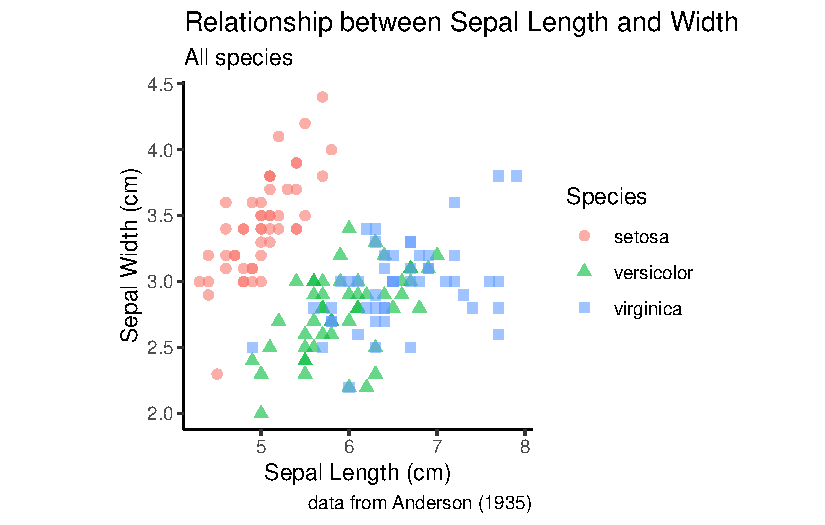
\includegraphics{_main_files/figure-latex/unnamed-chunk-2-1.pdf}

This precipitation data comes from the \href{https://www.climatologylab.org/terraclimate.html}{Terraclimate} product, giving modeled monthly spatial averages from 1958-present. Here, the values for each year have been summed, and then these annual values are then averaged to give average annual precipitation.

However, this particular raster covers all of Africa, which is way more data that we need. We'll import southern Africa borders shapefile to look at how we might subset it.

\begin{Shaded}
\begin{Highlighting}[]
\NormalTok{saBorders}\OtherTok{\textless{}{-}}\FunctionTok{st\_read}\NormalTok{(}\StringTok{"south\_africa\_border.shp"}\NormalTok{)}
\end{Highlighting}
\end{Shaded}

\begin{verbatim}
## Reading layer `south_africa_border' from data source 
##   `C:\Users\bdav_\Dropbox\Teaching\Spatial R Short Course\Bookdown\Exercise3\Exercise3\south_africa_border.shp' 
##   using driver `ESRI Shapefile'
## Simple feature collection with 3 features and 94 fields
## Geometry type: POLYGON
## Dimension:     XY
## Bounding box:  xmin: 16.46998 ymin: -34.82195 xmax: 32.89308 ymax: -22.12645
## Geodetic CRS:  WGS 84
\end{verbatim}

\begin{Shaded}
\begin{Highlighting}[]
\FunctionTok{plot}\NormalTok{(}\FunctionTok{st\_geometry}\NormalTok{(saBorders))}
\end{Highlighting}
\end{Shaded}

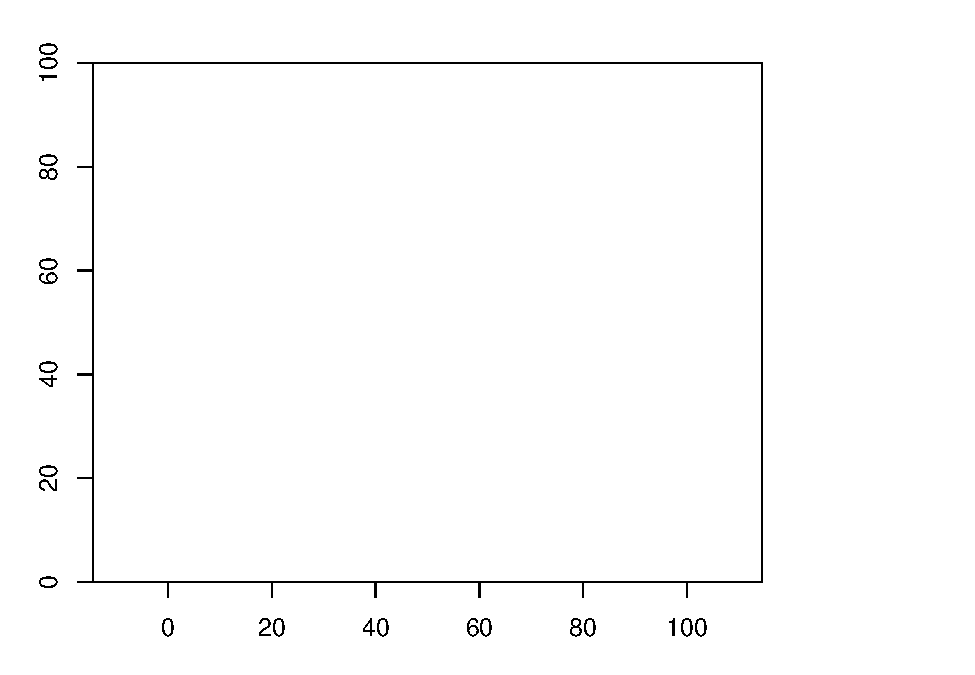
\includegraphics{_main_files/figure-latex/unnamed-chunk-3-1.pdf}

\hypertarget{crop-raster-with-vector-data}{%
\section{Crop raster with vector data}\label{crop-raster-with-vector-data}}

Now that we have a raster and a vector dataset, we'll use the latter to spatially subset the former. To do this, we will need the \texttt{crop} function.

\begin{Shaded}
\begin{Highlighting}[]
\CommentTok{\#Crop rainfall data to southern Africa}
\NormalTok{saAnnRain}\OtherTok{\textless{}{-}}\FunctionTok{crop}\NormalTok{(annRain,saBorders)}
\end{Highlighting}
\end{Shaded}

The first argument to the crop function is the raster we want crop (\texttt{annRain}). The second is the object we are using to set the new margins (\texttt{saBorders}).

Now we can take a look\ldots{}

\begin{Shaded}
\begin{Highlighting}[]
\CommentTok{\#Plot new raster and borders}
\FunctionTok{plot}\NormalTok{(saAnnRain)}
\FunctionTok{plot}\NormalTok{(}\FunctionTok{st\_geometry}\NormalTok{(saBorders),}\AttributeTok{add=}\NormalTok{T)}
\end{Highlighting}
\end{Shaded}

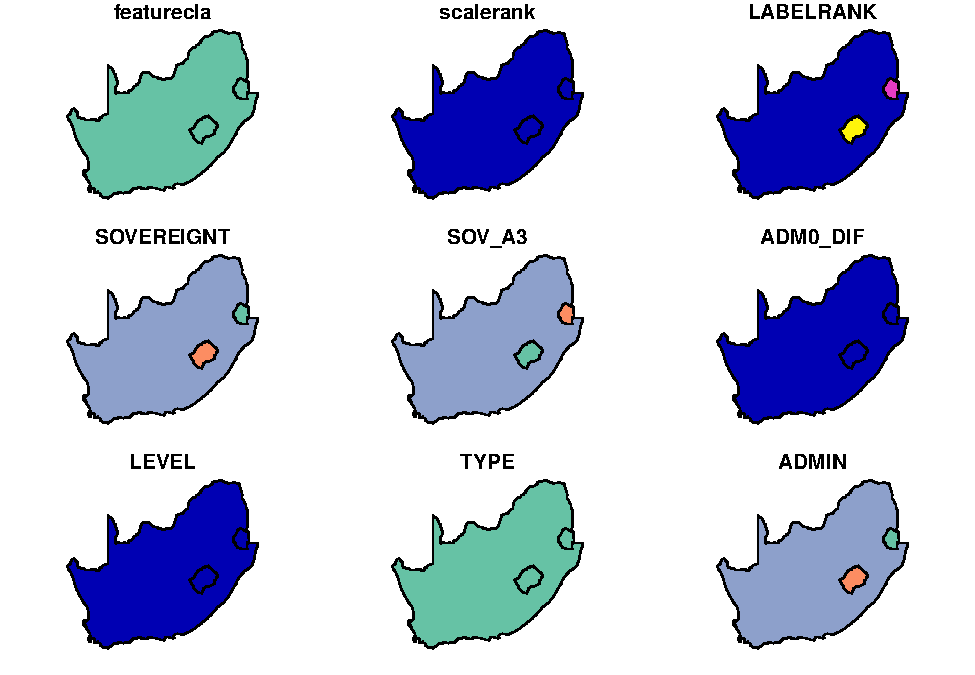
\includegraphics{_main_files/figure-latex/unnamed-chunk-5-1.pdf}

Hmmm\ldots{} this looks OK, but maybe not exactly what we wanted since the rainfall values extend beyond the area of interest. The main reason for this is that we used an \texttt{sf} object as the cropping object. When \texttt{terra} tries to do this, it can only crop to the extent of the object.

In order to crop more closely, we need to turn our \texttt{saBorders} object into a \texttt{terra} SpatVector object, which is a format \texttt{terra} uses to represnt vector data. We can use the \texttt{vect} function for this:

\begin{Shaded}
\begin{Highlighting}[]
\CommentTok{\#Turn sf object into a SpatVector dataset}
\NormalTok{saBordersSF}\OtherTok{\textless{}{-}}\FunctionTok{vect}\NormalTok{(saBorders)}
\NormalTok{saBordersSF}
\end{Highlighting}
\end{Shaded}

\begin{verbatim}
##  class       : SpatVector 
##  geometry    : polygons 
##  dimensions  : 3, 94  (geometries, attributes)
##  extent      : 16.46998, 32.89308, -34.82195, -22.12645  (xmin, xmax, ymin, ymax)
##  coord. ref. : lon/lat WGS 84 (EPSG:4326) 
##  names       :      featurecla scalerank LABELRANK   SOVEREIGNT SOV_A3 ADM0_DIF
##  type        :           <chr>     <int>     <int>        <chr>  <chr>    <int>
##  values      : Admin-0 country         0         2 South Africa    ZAF        0
##                Admin-0 country         0         4     eSwatini    SWZ        0
##                Admin-0 country         0         6      Lesotho    LSO        0
##  LEVEL              TYPE        ADMIN ADM0_A3 (and 84 more)
##  <int>             <chr>        <chr>   <chr>              
##      2 Sovereign country South Africa     ZAF              
##      2 Sovereign country     eSwatini     SWZ              
##      2 Sovereign country      Lesotho     LSO
\end{verbatim}

OK, now we have the borders as a SpatVector. We can plug this in and see what we get:

\begin{Shaded}
\begin{Highlighting}[]
\CommentTok{\#Crop rain data again with SpatVector}
\NormalTok{saAnnRain}\OtherTok{\textless{}{-}}\FunctionTok{crop}\NormalTok{(annRain,saBordersSF)}
\FunctionTok{plot}\NormalTok{(saAnnRain)}
\FunctionTok{plot}\NormalTok{(}\FunctionTok{st\_geometry}\NormalTok{(saBorders),}\AttributeTok{add=}\NormalTok{T)}
\end{Highlighting}
\end{Shaded}

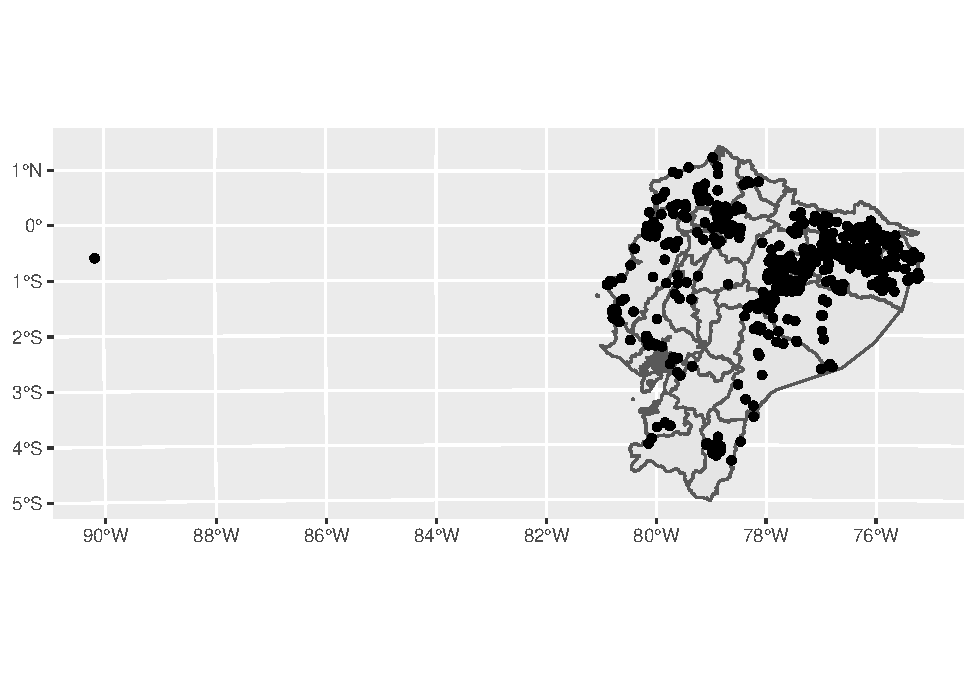
\includegraphics{_main_files/figure-latex/unnamed-chunk-7-1.pdf}

Still not quite there! The last step is that we need add the \texttt{mask} argument to the \texttt{crop} function and set it to true. This tells \texttt{crop} to take any values outside the cropping object and convert them to \texttt{NA} values.

\begin{Shaded}
\begin{Highlighting}[]
\CommentTok{\#Crop rain data again with SpatVector}
\NormalTok{saAnnRain}\OtherTok{\textless{}{-}}\FunctionTok{crop}\NormalTok{(annRain,saBordersSF,}\AttributeTok{mask=}\NormalTok{T)}
\FunctionTok{plot}\NormalTok{(saAnnRain)}
\FunctionTok{plot}\NormalTok{(}\FunctionTok{st\_geometry}\NormalTok{(saBorders),}\AttributeTok{add=}\NormalTok{T)}
\end{Highlighting}
\end{Shaded}

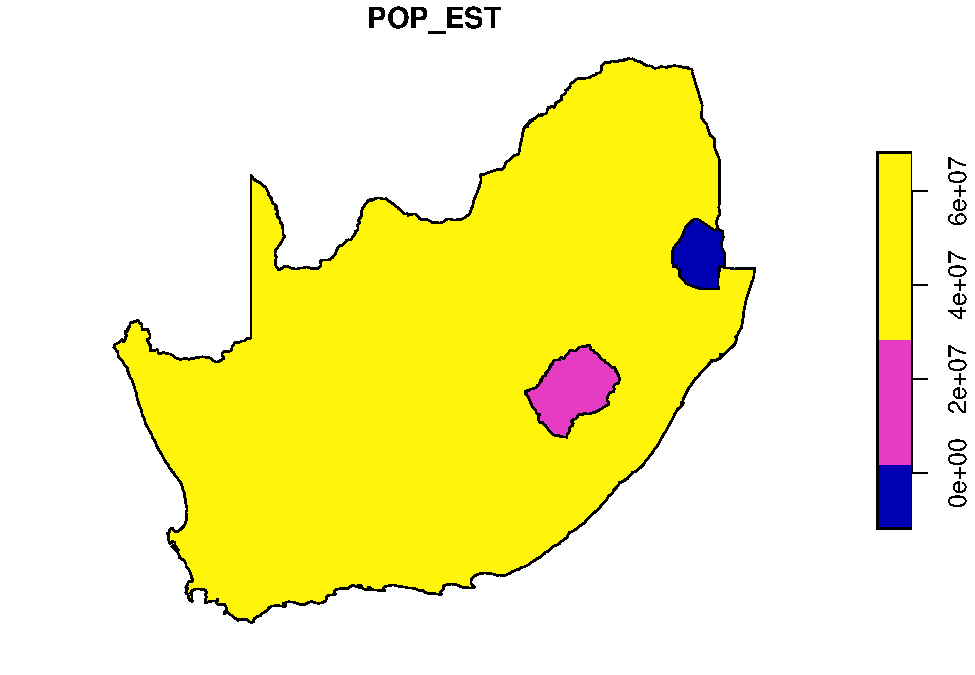
\includegraphics{_main_files/figure-latex/unnamed-chunk-8-1.pdf}

There we go! That looks much better. Let's use \texttt{global} to get a sense of the average and standard deviation on this new raster.

\begin{Shaded}
\begin{Highlighting}[]
\CommentTok{\#Get some stats}
\FunctionTok{global}\NormalTok{(saAnnRain,}\StringTok{"mean"}\NormalTok{)}
\end{Highlighting}
\end{Shaded}

\begin{verbatim}
##              mean
## africaAnnPPT  NaN
\end{verbatim}

\begin{Shaded}
\begin{Highlighting}[]
\FunctionTok{global}\NormalTok{(saAnnRain,}\StringTok{"sd"}\NormalTok{)}
\end{Highlighting}
\end{Shaded}

\begin{verbatim}
##               sd
## africaAnnPPT NaN
\end{verbatim}

Ack! When we see \texttt{NaN}, that stands for ``not a number''. That means R tried to do something mathematically impossible. The problem here is that, since we used \texttt{mask} to carve out our raster, there are now lots of \texttt{NA} values in the raster, and R can't calculate statistics when these values are present. We can use \texttt{na.rm} to get rid of them.

\begin{Shaded}
\begin{Highlighting}[]
\CommentTok{\#Get some stats}
\FunctionTok{global}\NormalTok{(saAnnRain,}\StringTok{"mean"}\NormalTok{,}\AttributeTok{na.rm=}\ConstantTok{TRUE}\NormalTok{)}
\end{Highlighting}
\end{Shaded}

\begin{verbatim}
##                 mean
## africaAnnPPT 439.047
\end{verbatim}

\begin{Shaded}
\begin{Highlighting}[]
\FunctionTok{global}\NormalTok{(saAnnRain,}\StringTok{"sd"}\NormalTok{,}\AttributeTok{na.rm=}\ConstantTok{TRUE}\NormalTok{)}
\end{Highlighting}
\end{Shaded}

\begin{verbatim}
##                    sd
## africaAnnPPT 228.5005
\end{verbatim}

\hypertarget{try-it-yourself}{%
\section{Try it yourself!}\label{try-it-yourself}}

\begin{itemize}
\tightlist
\item
  It's very easy to make histograms out of raster data. See if you can make a histogram out of the rainfall data for southern Africa and then all of Africa. How do they compare?
\item
  Can you create a boolean raster for places in southern Africa that get more than the mean rainfall?
\end{itemize}

\hypertarget{spatial-subsetting-raster-to-raster}{%
\chapter{Spatial subsetting: Raster to Raster}\label{spatial-subsetting-raster-to-raster}}

This time, we're going to use a raster data to perform a spatial subset on another raster. This should be a little more straightforward since we aren't trying to make \texttt{sf} and \texttt{terra} talk to eachother.

\hypertarget{add-more-raster-data}{%
\section{Add more raster data}\label{add-more-raster-data}}

Here we'll add another Terraclimate-derived dataset.

\begin{Shaded}
\begin{Highlighting}[]
\CommentTok{\#Import winter rainfall }
\NormalTok{winRain}\OtherTok{\textless{}{-}}\FunctionTok{rast}\NormalTok{(}\StringTok{"africaWinPPT.tif"}\NormalTok{)}

\CommentTok{\#Plot it}
\FunctionTok{plot}\NormalTok{(winRain)}
\end{Highlighting}
\end{Shaded}

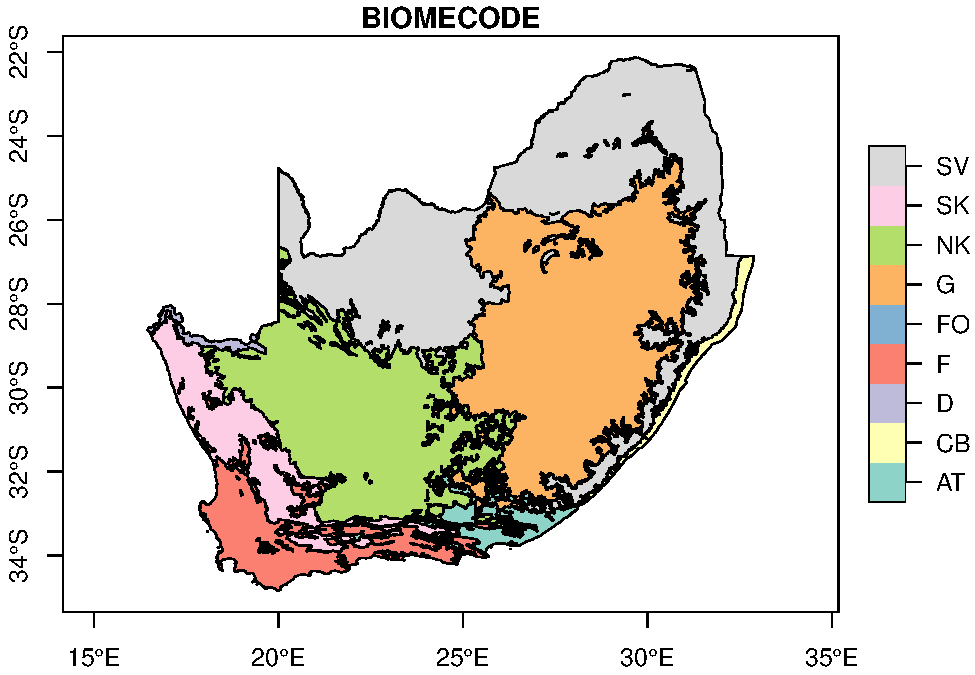
\includegraphics{_main_files/figure-latex/unnamed-chunk-11-1.pdf}

This is just like the annual average rainfall data, but only for the winter months (June, July, and August).

Since our annual rainfall data has already been cropped, we should be able to use that data to crop our new dataset.

\begin{Shaded}
\begin{Highlighting}[]
\CommentTok{\#Crop winter rain using annual rain}
\NormalTok{saWinRain}\OtherTok{\textless{}{-}}\FunctionTok{crop}\NormalTok{(winRain,saAnnRain,}\AttributeTok{mask=}\ConstantTok{TRUE}\NormalTok{)}

\CommentTok{\#Plot it}
\FunctionTok{plot}\NormalTok{(saWinRain)}
\end{Highlighting}
\end{Shaded}

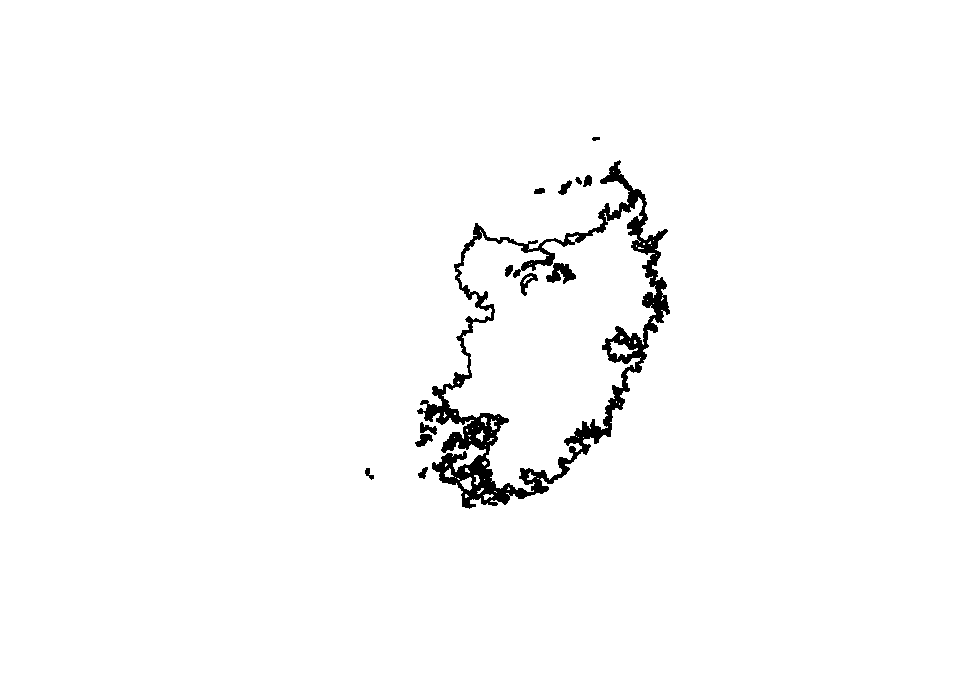
\includegraphics{_main_files/figure-latex/unnamed-chunk-12-1.pdf}
This again! The problem here is that the \texttt{mask} argument here only applies to a SpatVector object like we made in the previous section. If we want to use a raster to mask another raster, we need to call the \texttt{mask} function:

\begin{Shaded}
\begin{Highlighting}[]
\CommentTok{\#Crop it again}
\NormalTok{saWinRain}\OtherTok{\textless{}{-}}\FunctionTok{crop}\NormalTok{(winRain,saAnnRain)}

\CommentTok{\#Mask the winter rain data with the annual rain data}
\NormalTok{saWinRain}\OtherTok{\textless{}{-}}\FunctionTok{mask}\NormalTok{(saWinRain,saAnnRain)}

\CommentTok{\#Plot it}
\FunctionTok{plot}\NormalTok{(saWinRain)}
\end{Highlighting}
\end{Shaded}

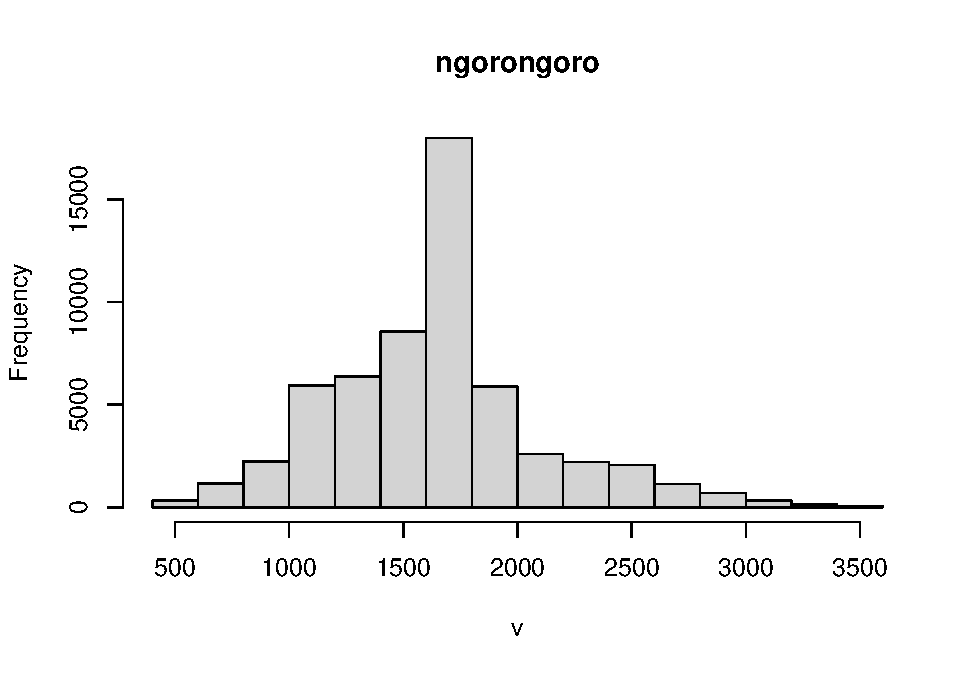
\includegraphics{_main_files/figure-latex/unnamed-chunk-13-1.pdf}
OK, great!

\hypertarget{raster-algebra-revisited}{%
\section{Raster algebra revisited}\label{raster-algebra-revisited}}

OK, for this last step, we want to know what percentage of an area's rainfall occurs in the winter. This will give us a sense of seasonality across southern Africa. To get this all we have to do is divide the winter rainfall values by the total annual values:

\begin{Shaded}
\begin{Highlighting}[]
\CommentTok{\#Get winter percentages}
\NormalTok{winRainPercent}\OtherTok{\textless{}{-}}\NormalTok{saWinRain}\SpecialCharTok{/}\NormalTok{saAnnRain}

\CommentTok{\#Plot it}
\FunctionTok{plot}\NormalTok{(winRainPercent)}
\end{Highlighting}
\end{Shaded}

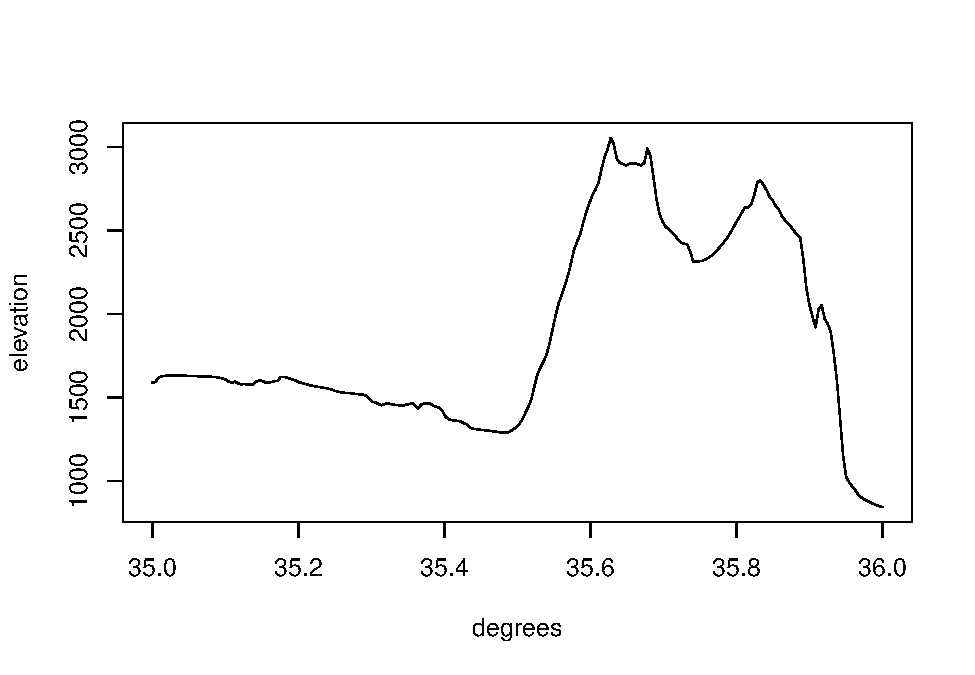
\includegraphics{_main_files/figure-latex/unnamed-chunk-14-1.pdf}

Cool! Hopefully from this map you can see southern Africa's very distinctive winter and summer rainfall zones.

\hypertarget{spatial-subsetting-vector-to-vector}{%
\chapter{Spatial subsetting: Vector to Vector}\label{spatial-subsetting-vector-to-vector}}

The last spatial subsetting we'll do is using one vector to subset another.

\hypertarget{convert-table-data-to-vector-data}{%
\section{Convert table data to vector data}\label{convert-table-data-to-vector-data}}

First let's bring in some table data with spatial coordinates:

\begin{Shaded}
\begin{Highlighting}[]
\NormalTok{micro}\OtherTok{\textless{}{-}}\FunctionTok{read.csv}\NormalTok{(}\StringTok{"micromammals.csv"}\NormalTok{)}
\FunctionTok{head}\NormalTok{(micro)}
\end{Highlighting}
\end{Shaded}

\begin{verbatim}
##                         Site Abbreviation Latitude Longitude CODE        ORDER
## 1 100 Elliott Street Kokstad          ESK   -30.54     29.41 CCYA SORICOMORPHA
## 2 100 Elliott Street Kokstad          ESK   -30.54     29.41 CFLA SORICOMORPHA
## 3 100 Elliott Street Kokstad          ESK   -30.54     29.41 DINC     RODENTIA
## 4 100 Elliott Street Kokstad          ESK   -30.54     29.41 MMIN     RODENTIA
## 5 100 Elliott Street Kokstad          ESK   -30.54     29.41 MMUS     RODENTIA
## 6 100 Elliott Street Kokstad          ESK   -30.54     29.41 MNAT     RODENTIA
##      FAMILY    SUBFAMILY     GENUS       SPECIES                   COMMONNAME
## 1 Soricidae Crocidurinae Crocidura        cyanea      Reddish-gray Musk Shrew
## 2 Soricidae Crocidurinae Crocidura    flavescens       Greater Red Musk Shrew
## 3   Muridae      Murinae  Dasymys  incomtus s.l.               Common Dasymys
## 4   Muridae      Murinae      Mus     minutoides Southern African Pygmy Mouse
## 5   Muridae      Murinae      Mus       musculus                  House Mouse
## 6   Muridae      Murinae Mastomys     natalensis               Natal Mastomys
\end{verbatim}

These are modern micromammal occurrences that were used in this paper:

Faith, J. Tyler, Brian M. Chase, and D. Margaret Avery. 2019. ``Late Quaternary Micromammals and the Precipitation History of the Southern Cape, South Africa.'' Quaternary Research 91 (2): 848--60. \url{https://doi.org/10.1017/qua.2018.105}.

The information includes the site, the coordinates, and the species encountered. In order to make use of it in our analysis, we need to turn it into vector data.

\begin{Shaded}
\begin{Highlighting}[]
\NormalTok{microSF}\OtherTok{\textless{}{-}}\FunctionTok{st\_as\_sf}\NormalTok{(micro,}\AttributeTok{coords=}\FunctionTok{c}\NormalTok{(}\StringTok{"Longitude"}\NormalTok{,}\StringTok{"Latitude"}\NormalTok{),}\AttributeTok{crs=}\DecValTok{4326}\NormalTok{)}
\FunctionTok{plot}\NormalTok{(}\FunctionTok{st\_geometry}\NormalTok{(microSF),}\AttributeTok{axes=}\NormalTok{T)}
\end{Highlighting}
\end{Shaded}

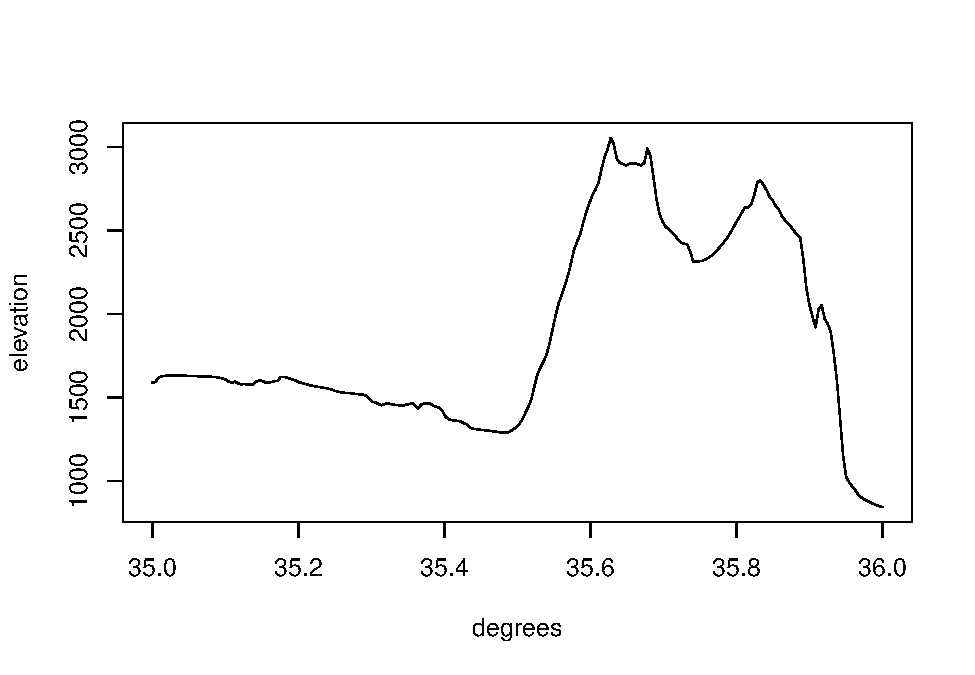
\includegraphics{_main_files/figure-latex/unnamed-chunk-16-1.pdf}

\hypertarget{cropping-vector-to-vector}{%
\section{Cropping vector to vector}\label{cropping-vector-to-vector}}

The way to crop one vector dataset with another is to use the \texttt{st\_crop} function.

\begin{Shaded}
\begin{Highlighting}[]
\CommentTok{\#Crop micromammal dataset to southern Africa}
\NormalTok{micromammals}\OtherTok{\textless{}{-}}\FunctionTok{st\_crop}\NormalTok{(microSF,saBorders)}
\end{Highlighting}
\end{Shaded}

\begin{verbatim}
## Warning: attribute variables are assumed to be spatially constant throughout all
## geometries
\end{verbatim}

Note that warning, but don't worry too much about it. This is \texttt{terra} reminding you that, by subsetting this way, your are assuming that the attributes are spatially constant.

Imagine if you were using this function to crop a polygon that represented grassland vegetation. This wouldn't be problematic, because the cropped polygon would still be grassland. However, now imagine that you used it to crop the polygon for Lesotho, which contains a population estimate. That population estimate would no longer be valid for the cropped section of Lesotho.

Here, we're not really worried about this because we're pruning points, so there isn't any cutting of individual features. Let's take a look.

\begin{Shaded}
\begin{Highlighting}[]
\CommentTok{\#Plot borders and micromammals}
\FunctionTok{plot}\NormalTok{(}\FunctionTok{st\_geometry}\NormalTok{(saBorders),}\AttributeTok{axes=}\NormalTok{T)}
\FunctionTok{plot}\NormalTok{(}\FunctionTok{st\_geometry}\NormalTok{(micromammals),}\AttributeTok{add=}\NormalTok{T)}
\end{Highlighting}
\end{Shaded}

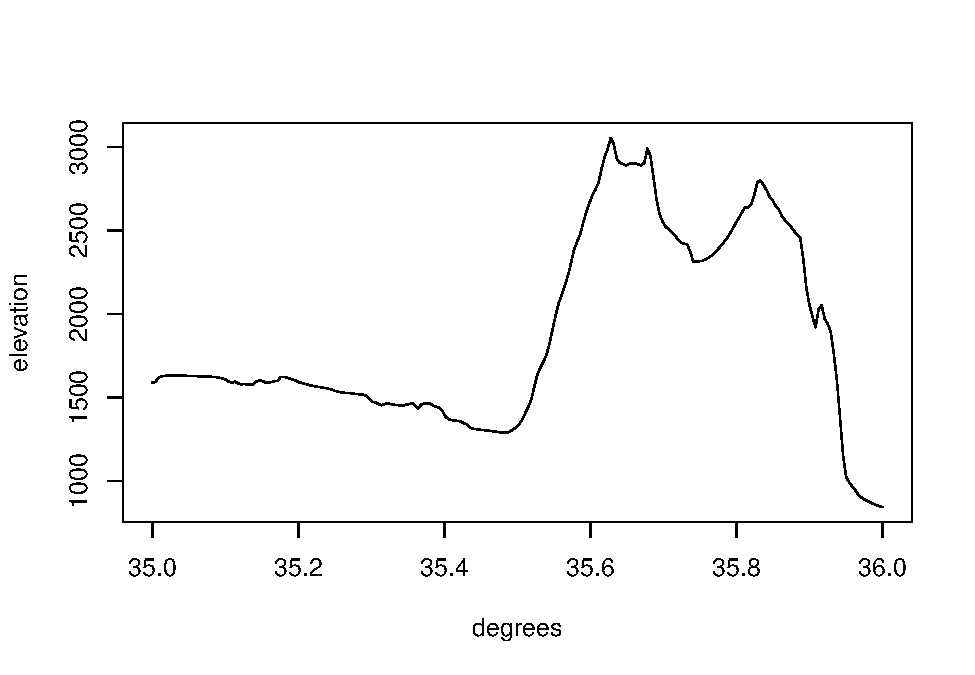
\includegraphics{_main_files/figure-latex/unnamed-chunk-18-1.pdf}
Looks good!

\hypertarget{try-it-yourself-1}{%
\section{Try it yourself}\label{try-it-yourself-1}}

\begin{itemize}
\tightlist
\item
  Create a plot that shows the borders, but instead of just the micromammal point locations, plot them by genus (hint: this may involve square brackets).
\item
  Change the symbol shape with the \texttt{pch} argument (it takes an integer and defaults to 1).
\end{itemize}

\hypertarget{spatial-sampling}{%
\chapter{Spatial Sampling}\label{spatial-sampling}}

For this final step, we're going to use our micromammal vector data to sample our raster data on rainfall seasonality.

\hypertarget{extract-point-values}{%
\section{Extract point values}\label{extract-point-values}}

To accomplish this, we need to use \texttt{extract}, which we've seen before. In that instance, we used a matrix of XY values. Here, we want to use the locations of our micromammals. To use it here with our SpatRaster object, we need to make it into a SpatVector object with \texttt{vect}.

\begin{Shaded}
\begin{Highlighting}[]
\NormalTok{winRainMM}\OtherTok{\textless{}{-}}\FunctionTok{extract}\NormalTok{(winRainPercent,}\FunctionTok{vect}\NormalTok{(micromammals))}
\NormalTok{winRainMM}
\end{Highlighting}
\end{Shaded}

\begin{verbatim}
##        ID africaWinPPT
## 1       1   0.17195767
## 2       2   0.17195767
## 3       3   0.17195767
## 4       4   0.17195767
## 5       5   0.17195767
## 6       6   0.17195767
## 7       7   0.17195767
## 8       8   0.17195767
## 9       9   0.17195767
## 10     10   0.17195767
## 11     11   0.14122682
## 12     12   0.14122682
## 13     13   0.14122682
## 14     14   0.14122682
## 15     15   0.14122682
## 16     16   0.14122682
## 17     17   0.14122682
## 18     18   0.14122682
## 19     19   0.14122682
## 20     20   0.14122682
## 21     21   0.14122682
## 22     22   0.14122682
## 23     23   0.14122682
## 24     24   0.13150289
## 25     25   0.13150289
## 26     26   0.13150289
## 27     27   0.13150289
## 28     28   0.13150289
## 29     29   0.13150289
## 30     30   0.13150289
## 31     31   0.13150289
## 32     32   0.13150289
## 33     33   0.09735974
## 34     34   0.09735974
## 35     35   0.09735974
## 36     36   0.09735974
## 37     37   0.09735974
## 38     38   0.09735974
## 39     39   0.63436123
## 40     40   0.63436123
## 41     41   0.63436123
## 42     42   0.63436123
## 43     43   0.63436123
## 44     44   0.63436123
## 45     45   0.63436123
## 46     46   0.63436123
## 47     47   0.63436123
## 48     48   0.63436123
## 49     49   0.63436123
## 50     50   0.63436123
## 51     51   0.63436123
## 52     52   0.63436123
## 53     53   0.63436123
## 54     54   0.63436123
## 55     55   0.63436123
## 56     56   0.63436123
## 57     57   0.63436123
## 58     58   0.63436123
## 59     59   0.63436123
## 60     60   0.63436123
## 61     61   0.63436123
## 62     62   0.63436123
## 63     63   0.63436123
## 64     64   0.63436123
## 65     65   0.63436123
## 66     66   0.63436123
## 67     67   0.63436123
## 68     68   0.63436123
## 69     69   0.63436123
## 70     70   0.60000000
## 71     71   0.60000000
## 72     72   0.60000000
## 73     73   0.60000000
## 74     74   0.60000000
## 75     75   0.60000000
## 76     76   0.60000000
## 77     77   0.60000000
## 78     78   0.60000000
## 79     79   0.60000000
## 80     80   0.60000000
## 81     81   0.60000000
## 82     82   0.60000000
## 83     83   0.70895522
## 84     84   0.70895522
## 85     85   0.70895522
## 86     86   0.70895522
## 87     87   0.70895522
## 88     88   0.70895522
## 89     89   0.70895522
## 90     90   0.70895522
## 91     91   0.70895522
## 92     92   0.70895522
## 93     93   0.70895522
## 94     94   0.70895522
## 95     95   0.70895522
## 96     96   0.70895522
## 97     97   0.70895522
## 98     98   0.70895522
## 99     99   0.70895522
## 100   100   0.70895522
## 101   101   0.53664303
## 102   102   0.53664303
## 103   103   0.53664303
## 104   104   0.53664303
## 105   105   0.53664303
## 106   106   0.53664303
## 107   107   0.53664303
## 108   108   0.53664303
## 109   109   0.18820577
## 110   110   0.18820577
## 111   111   0.18820577
## 112   112   0.18820577
## 113   113   0.18820577
## 114   114   0.18820577
## 115   115   0.18820577
## 116   116   0.17977528
## 117   117   0.17977528
## 118   118   0.17977528
## 119   119   0.05405405
## 120   120   0.05405405
## 121   121   0.05405405
## 122   122   0.05405405
## 123   123   0.05405405
## 124   124   0.05405405
## 125   125   0.57986871
## 126   126   0.57986871
## 127   127   0.57986871
## 128   128   0.57986871
## 129   129   0.57986871
## 130   130   0.57986871
## 131   131   0.57986871
## 132   132   0.57986871
## 133   133   0.57986871
## 134   134   0.57986871
## 135   135   0.09001637
## 136   136   0.09001637
## 137   137   0.09001637
## 138   138   0.09001637
## 139   139   0.09001637
## 140   140   0.09001637
## 141   141   0.09001637
## 142   142   0.09001637
## 143   143   0.09001637
## 144   144   0.09001637
## 145   145   0.09001637
## 146   146   0.09001637
## 147   147   0.09001637
## 148   148   0.09001637
## 149   149   0.09001637
## 150   150   0.09001637
## 151   151   0.09001637
## 152   152   0.09001637
## 153   153   0.09001637
## 154   154   0.13785047
## 155   155   0.13785047
## 156   156   0.13785047
## 157   157   0.13785047
## 158   158   0.13785047
## 159   159   0.13785047
## 160   160   0.13785047
## 161   161   0.13785047
## 162   162   0.13785047
## 163   163   0.13785047
## 164   164   0.13785047
## 165   165   0.63348416
## 166   166   0.63348416
## 167   167   0.63348416
## 168   168   0.63348416
## 169   169   0.63348416
## 170   170   0.63348416
## 171   171   0.63348416
## 172   172   0.63348416
## 173   173   0.63348416
## 174   174   0.63348416
## 175   175   0.63348416
## 176   176   0.60606061
## 177   177   0.60606061
## 178   178   0.60606061
## 179   179   0.60606061
## 180   180   0.60606061
## 181   181   0.60606061
## 182   182   0.60606061
## 183   183   0.60606061
## 184   184   0.46351931
## 185   185   0.46351931
## 186   186   0.46351931
## 187   187   0.46351931
## 188   188   0.46351931
## 189   189   0.46351931
## 190   190   0.46351931
## 191   191   0.46351931
## 192   192   0.46351931
## 193   193   0.46351931
## 194   194   0.46351931
## 195   195   0.46351931
## 196   196   0.46351931
## 197   197   0.26937269
## 198   198   0.26937269
## 199   199   0.26937269
## 200   200   0.26937269
## 201   201   0.26937269
## 202   202   0.26937269
## 203   203   0.26937269
## 204   204   0.26937269
## 205   205   0.26937269
## 206   206   0.49870130
## 207   207   0.49870130
## 208   208   0.49870130
## 209   209   0.49870130
## 210   210   0.49870130
## 211   211   0.49870130
## 212   212   0.49870130
## 213   213   0.49870130
## 214   214   0.49870130
## 215   215   0.49870130
## 216   216   0.49870130
## 217   217   0.49870130
## 218   218   0.49870130
## 219   219   0.49870130
## 220   220   0.49870130
## 221   221   0.49870130
## 222   222   0.49870130
## 223   223   0.49870130
## 224   224   0.49870130
## 225   225   0.49870130
## 226   226   0.49870130
## 227   227   0.49870130
## 228   228   0.49870130
## 229   229   0.49870130
## 230   230   0.49870130
## 231   231   0.49870130
## 232   232   0.49870130
## 233   233   0.49870130
## 234   234   0.49870130
## 235   235   0.49870130
## 236   236   0.49870130
## 237   237   0.49870130
## 238   238   0.49870130
## 239   239   0.49870130
## 240   240   0.49870130
## 241   241   0.56511628
## 242   242   0.56511628
## 243   243   0.56511628
## 244   244   0.56511628
## 245   245   0.56511628
## 246   246   0.56511628
## 247   247   0.56511628
## 248   248   0.56511628
## 249   249   0.56511628
## 250   250   0.56511628
## 251   251   0.56511628
## 252   252   0.56511628
## 253   253   0.69082126
## 254   254   0.69082126
## 255   255   0.69082126
## 256   256   0.69082126
## 257   257   0.69082126
## 258   258   0.69082126
## 259   259   0.69082126
## 260   260   0.69082126
## 261   261   0.69082126
## 262   262   0.69082126
## 263   263   0.69082126
## 264   264   0.69082126
## 265   265   0.69082126
## 266   266   0.69082126
## 267   267   0.69082126
## 268   268   0.26070039
## 269   269   0.26070039
## 270   270   0.26070039
## 271   271   0.26070039
## 272   272   0.26070039
## 273   273   0.26070039
## 274   274   0.26070039
## 275   275   0.26070039
## 276   276   0.56097561
## 277   277   0.56097561
## 278   278   0.56097561
## 279   279   0.56097561
## 280   280   0.56097561
## 281   281   0.56097561
## 282   282   0.56097561
## 283   283   0.56097561
## 284   284   0.53664303
## 285   285   0.53664303
## 286   286   0.53664303
## 287   287   0.53664303
## 288   288   0.53664303
## 289   289   0.53664303
## 290   290   0.53664303
## 291   291   0.53664303
## 292   292   0.53664303
## 293   293   0.53664303
## 294   294   0.53664303
## 295   295   0.53664303
## 296   296   0.53664303
## 297   297   0.06433566
## 298   298   0.06433566
## 299   299   0.06433566
## 300   300   0.06433566
## 301   301   0.06433566
## 302   302   0.06433566
## 303   303   0.06433566
## 304   304   0.06433566
## 305   305   0.57048458
## 306   306   0.57048458
## 307   307   0.57048458
## 308   308   0.57048458
## 309   309   0.57048458
## 310   310   0.57048458
## 311   311   0.57048458
## 312   312   0.57048458
## 313   313   0.57048458
## 314   314   0.57048458
## 315   315   0.57048458
## 316   316   0.57048458
## 317   317   0.57048458
## 318   318   0.57048458
## 319   319   0.57048458
## 320   320   0.57048458
## 321   321   0.57048458
## 322   322   0.57048458
## 323   323   0.57048458
## 324   324   0.57048458
## 325   325   0.57048458
## 326   326   0.57048458
## 327   327   0.46850394
## 328   328   0.46850394
## 329   329   0.46850394
## 330   330   0.46850394
## 331   331   0.46850394
## 332   332   0.46850394
## 333   333   0.46850394
## 334   334   0.46850394
## 335   335   0.46850394
## 336   336   0.66101695
## 337   337   0.66101695
## 338   338   0.66101695
## 339   339   0.66101695
## 340   340   0.66101695
## 341   341   0.66101695
## 342   342   0.66101695
## 343   343   0.66101695
## 344   344   0.66101695
## 345   345   0.66101695
## 346   346   0.63000000
## 347   347   0.63000000
## 348   348   0.63000000
## 349   349   0.63000000
## 350   350   0.63000000
## 351   351   0.63000000
## 352   352   0.63000000
## 353   353   0.63000000
## 354   354   0.63000000
## 355   355   0.63000000
## 356   356   0.63000000
## 357   357   0.60128617
## 358   358   0.60128617
## 359   359   0.60128617
## 360   360   0.60128617
## 361   361   0.60128617
## 362   362   0.60128617
## 363   363   0.60128617
## 364   364   0.60128617
## 365   365   0.60128617
## 366   366   0.34558824
## 367   367   0.34558824
## 368   368   0.34558824
## 369   369   0.34558824
## 370   370   0.34558824
## 371   371   0.34558824
## 372   372   0.34558824
## 373   373   0.34558824
## 374   374   0.51068376
## 375   375   0.51068376
## 376   376   0.51068376
## 377   377   0.51068376
## 378   378   0.51068376
## 379   379   0.51068376
## 380   380   0.51068376
## 381   381   0.51068376
## 382   382   0.51068376
## 383   383   0.51068376
## 384   384   0.51068376
## 385   385   0.51068376
## 386   386   0.51068376
## 387   387   0.51068376
## 388   388   0.51068376
## 389   389   0.51068376
## 390   390           NA
## 391   391           NA
## 392   392           NA
## 393   393           NA
## 394   394           NA
## 395   395           NA
## 396   396           NA
## 397   397           NA
## 398   398           NA
## 399   399           NA
## 400   400   0.55000000
## 401   401   0.55000000
## 402   402   0.55000000
## 403   403   0.55000000
## 404   404   0.55000000
## 405   405   0.55000000
## 406   406   0.55000000
## 407   407   0.55000000
## 408   408   0.55000000
## 409   409   0.55000000
## 410   410   0.55000000
## 411   411   0.55000000
## 412   412   0.22916667
## 413   413   0.22916667
## 414   414   0.22916667
## 415   415   0.22916667
## 416   416   0.22916667
## 417   417   0.22916667
## 418   418   0.22916667
## 419   419   0.22916667
## 420   420   0.22916667
## 421   421   0.22916667
## 422   422   0.22916667
## 423   423   0.22916667
## 424   424   0.22916667
## 425   425   0.22916667
## 426   426   0.22916667
## 427   427   0.22916667
## 428   428   0.20526316
## 429   429   0.20526316
## 430   430   0.20526316
## 431   431   0.20526316
## 432   432   0.20526316
## 433   433   0.20526316
## 434   434   0.20526316
## 435   435   0.20526316
## 436   436   0.20526316
## 437   437   0.20526316
## 438   438   0.20526316
## 439   439   0.20526316
## 440   440   0.21904762
## 441   441   0.21904762
## 442   442   0.21904762
## 443   443   0.21904762
## 444   444   0.21904762
## 445   445   0.21904762
## 446   446   0.21904762
## 447   447   0.21904762
## 448   448   0.21904762
## 449   449   0.21904762
## 450   450   0.21904762
## 451   451   0.21904762
## 452   452   0.21904762
## 453   453   0.21904762
## 454   454   0.21904762
## 455   455   0.21904762
## 456   456   0.21904762
## 457   457   0.21904762
## 458   458   0.12165450
## 459   459   0.12165450
## 460   460   0.12165450
## 461   461   0.12165450
## 462   462   0.12165450
## 463   463   0.12165450
## 464   464   0.14973262
## 465   465   0.14973262
## 466   466   0.14973262
## 467   467   0.14973262
## 468   468   0.14973262
## 469   469   0.14973262
## 470   470   0.14973262
## 471   471   0.14973262
## 472   472   0.14973262
## 473   473   0.14973262
## 474   474   0.14973262
## 475   475   0.14973262
## 476   476   0.14973262
## 477   477   0.14973262
## 478   478   0.14973262
## 479   479   0.14973262
## 480   480   0.14973262
## 481   481   0.44941957
## 482   482   0.44941957
## 483   483   0.44941957
## 484   484   0.44941957
## 485   485   0.44941957
## 486   486   0.44941957
## 487   487   0.44941957
## 488   488   0.44941957
## 489   489   0.44941957
## 490   490   0.44941957
## 491   491   0.44941957
## 492   492   0.08269720
## 493   493   0.08269720
## 494   494   0.08269720
## 495   495   0.08269720
## 496   496   0.08269720
## 497   497   0.08269720
## 498   498   0.08269720
## 499   499   0.08269720
## 500   500   0.08269720
## 501   501   0.08269720
## 502   502   0.08269720
## 503   503   0.08269720
## 504   504   0.08269720
## 505   505   0.08269720
## 506   506   0.08269720
## 507   507   0.08269720
## 508   508   0.08269720
## 509   509   0.08269720
## 510   510   0.08269720
## 511   511   0.08269720
## 512   512   0.08269720
## 513   513   0.08269720
## 514   514   0.08269720
## 515   515   0.08269720
## 516   516   0.08269720
## 517   517   0.08269720
## 518   518   0.12554745
## 519   519   0.12554745
## 520   520   0.12554745
## 521   521   0.12554745
## 522   522   0.12554745
## 523   523   0.12554745
## 524   524   0.12554745
## 525   525   0.12554745
## 526   526   0.12554745
## 527   527   0.12554745
## 528   528   0.12554745
## 529   529   0.28892734
## 530   530   0.28892734
## 531   531   0.28892734
## 532   532   0.28892734
## 533   533   0.28892734
## 534   534   0.28892734
## 535   535   0.28892734
## 536   536   0.28892734
## 537   537   0.28892734
## 538   538   0.28892734
## 539   539   0.28892734
## 540   540   0.28892734
## 541   541   0.28892734
## 542   542           NA
## 543   543           NA
## 544   544           NA
## 545   545           NA
## 546   546           NA
## 547   547           NA
## 548   548           NA
## 549   549           NA
## 550   550           NA
## 551   551           NA
## 552   552           NA
## 553   553           NA
## 554   554           NA
## 555   555           NA
## 556   556           NA
## 557   557           NA
## 558   558           NA
## 559   559           NA
## 560   560           NA
## 561   561           NA
## 562   562           NA
## 563   563           NA
## 564   564           NA
## 565   565           NA
## 566   566           NA
## 567   567           NA
## 568   568           NA
## 569   569           NA
## 570   570           NA
## 571   571           NA
## 572   572           NA
## 573   573           NA
## 574   574   0.37030411
## 575   575   0.37030411
## 576   576   0.37030411
## 577   577   0.37030411
## 578   578   0.37030411
## 579   579   0.37030411
## 580   580   0.37030411
## 581   581   0.37030411
## 582   582   0.37030411
## 583   583   0.37030411
## 584   584   0.37030411
## 585   585   0.37030411
## 586   586   0.37030411
## 587   587   0.37030411
## 588   588   0.37030411
## 589   589   0.37030411
## 590   590   0.37030411
## 591   591   0.15333333
## 592   592   0.15333333
## 593   593   0.15333333
## 594   594   0.15333333
## 595   595   0.15333333
## 596   596   0.15333333
## 597   597   0.15333333
## 598   598   0.15333333
## 599   599   0.15333333
## 600   600   0.15333333
## 601   601   0.15333333
## 602   602   0.15333333
## 603   603   0.13119534
## 604   604   0.13119534
## 605   605   0.13119534
## 606   606   0.13119534
## 607   607   0.13119534
## 608   608   0.13119534
## 609   609   0.13119534
## 610   610   0.13119534
## 611   611   0.13119534
## 612   612   0.13119534
## 613   613   0.13119534
## 614   614   0.44941957
## 615   615   0.44941957
## 616   616   0.44941957
## 617   617   0.44941957
## 618   618   0.44941957
## 619   619   0.44941957
## 620   620   0.44941957
## 621   621   0.44941957
## 622   622   0.44941957
## 623   623   0.44941957
## 624   624   0.44941957
## 625   625   0.44941957
## 626   626   0.44941957
## 627   627   0.44941957
## 628   628   0.44941957
## 629   629   0.44941957
## 630   630   0.44941957
## 631   631   0.44941957
## 632   632   0.44941957
## 633   633   0.56451613
## 634   634   0.56451613
## 635   635   0.56451613
## 636   636   0.56451613
## 637   637   0.56451613
## 638   638   0.56451613
## 639   639   0.56451613
## 640   640   0.56451613
## 641   641   0.56451613
## 642   642   0.56451613
## 643   643   0.56451613
## 644   644   0.23883495
## 645   645   0.23883495
## 646   646   0.23883495
## 647   647   0.23883495
## 648   648   0.23883495
## 649   649   0.23883495
## 650   650   0.23618090
## 651   651   0.23618090
## 652   652   0.23618090
## 653   653   0.23618090
## 654   654   0.23618090
## 655   655   0.23618090
## 656   656   0.23618090
## 657   657   0.23618090
## 658   658   0.23618090
## 659   659   0.23618090
## 660   660   0.23618090
## 661   661   0.23618090
## 662   662   0.23618090
## 663   663   0.14423077
## 664   664   0.14423077
## 665   665   0.14423077
## 666   666   0.14423077
## 667   667   0.14423077
## 668   668   0.14423077
## 669   669   0.14423077
## 670   670   0.14423077
## 671   671   0.14423077
## 672   672   0.14423077
## 673   673   0.14423077
## 674   674   0.14423077
## 675   675   0.14423077
## 676   676   0.14423077
## 677   677   0.31025300
## 678   678   0.31025300
## 679   679   0.31025300
## 680   680   0.31025300
## 681   681   0.31025300
## 682   682   0.31025300
## 683   683   0.31025300
## 684   684   0.31025300
## 685   685   0.31025300
## 686   686   0.31025300
## 687   687   0.31025300
## 688   688   0.31025300
## 689   689   0.21637427
## 690   690   0.21637427
## 691   691   0.21637427
## 692   692   0.21637427
## 693   693   0.21637427
## 694   694   0.21637427
## 695   695   0.21637427
## 696   696   0.56302521
## 697   697   0.56302521
## 698   698   0.56302521
## 699   699   0.56302521
## 700   700   0.60000000
## 701   701   0.60000000
## 702   702   0.60000000
## 703   703   0.60000000
## 704   704   0.60000000
## 705   705   0.60000000
## 706   706   0.60000000
## 707   707   0.60000000
## 708   708   0.60000000
## 709   709   0.60000000
## 710   710   0.60000000
## 711   711   0.60000000
## 712   712   0.38283828
## 713   713   0.38283828
## 714   714   0.38283828
## 715   715   0.38283828
## 716   716   0.38283828
## 717   717   0.38283828
## 718   718   0.38283828
## 719   719   0.38283828
## 720   720   0.38283828
## 721   721   0.38283828
## 722   722   0.38283828
## 723   723   0.38283828
## 724   724   0.38283828
## 725   725   0.38283828
## 726   726   0.38283828
## 727   727   0.38283828
## 728   728   0.38283828
## 729   729   0.38283828
## 730   730   0.22033898
## 731   731   0.22033898
## 732   732   0.22033898
## 733   733   0.22033898
## 734   734   0.22033898
## 735   735   0.22033898
## 736   736   0.22033898
## 737   737   0.22033898
## 738   738   0.22033898
## 739   739   0.22033898
## 740   740   0.22033898
## 741   741   0.22033898
## 742   742   0.22033898
## 743   743   0.22033898
## 744   744   0.22033898
## 745   745   0.22033898
## 746   746   0.13769124
## 747   747   0.13769124
## 748   748   0.13769124
## 749   749   0.13769124
## 750   750   0.13769124
## 751   751   0.13769124
## 752   752   0.13769124
## 753   753   0.13769124
## 754   754   0.13769124
## 755   755   0.13769124
## 756   756   0.13769124
## 757   757   0.13769124
## 758   758   0.13769124
## 759   759   0.13769124
## 760   760   0.13769124
## 761   761   0.19235512
## 762   762   0.19235512
## 763   763   0.19235512
## 764   764   0.19235512
## 765   765   0.19235512
## 766   766   0.19235512
## 767   767   0.19235512
## 768   768   0.19235512
## 769   769   0.19235512
## 770   770   0.55607477
## 771   771   0.55607477
## 772   772   0.55607477
## 773   773   0.55607477
## 774   774   0.55607477
## 775   775   0.55607477
## 776   776   0.55607477
## 777   777   0.55607477
## 778   778   0.55607477
## 779   779   0.55607477
## 780   780   0.55607477
## 781   781   0.55607477
## 782   782   0.55607477
## 783   783   0.55607477
## 784   784   0.55607477
## 785   785   0.55607477
## 786   786   0.55607477
## 787   787   0.55607477
## 788   788   0.15862069
## 789   789   0.15862069
## 790   790   0.15862069
## 791   791   0.15862069
## 792   792   0.21693122
## 793   793   0.21693122
## 794   794   0.21693122
## 795   795   0.21693122
## 796   796   0.21693122
## 797   797   0.21693122
## 798   798   0.21693122
## 799   799   0.21693122
## 800   800   0.21693122
## 801   801   0.21693122
## 802   802   0.21693122
## 803   803   0.21693122
## 804   804   0.21693122
## 805   805   0.21693122
## 806   806   0.21693122
## 807   807   0.22699387
## 808   808   0.22699387
## 809   809   0.22699387
## 810   810   0.22699387
## 811   811   0.22699387
## 812   812   0.22699387
## 813   813   0.22699387
## 814   814   0.22699387
## 815   815   0.22699387
## 816   816   0.73282443
## 817   817   0.73282443
## 818   818   0.73282443
## 819   819   0.73282443
## 820   820   0.73282443
## 821   821   0.73282443
## 822   822   0.73282443
## 823   823   0.73282443
## 824   824   0.73282443
## 825   825   0.73282443
## 826   826   0.73282443
## 827   827   0.73282443
## 828   828   0.73282443
## 829   829           NA
## 830   830           NA
## 831   831           NA
## 832   832           NA
## 833   833           NA
## 834   834           NA
## 835   835           NA
## 836   836           NA
## 837   837           NA
## 838   838           NA
## 839   839           NA
## 840   840           NA
## 841   841   0.11639344
## 842   842   0.11639344
## 843   843   0.11639344
## 844   844   0.11639344
## 845   845   0.11639344
## 846   846   0.11639344
## 847   847   0.11639344
## 848   848   0.11639344
## 849   849   0.11639344
## 850   850   0.11639344
## 851   851   0.11639344
## 852   852   0.11639344
## 853   853   0.11639344
## 854   854   0.11639344
## 855   855   0.11639344
## 856   856   0.11639344
## 857   857   0.11639344
## 858   858   0.11639344
## 859   859   0.57558140
## 860   860   0.57558140
## 861   861   0.57558140
## 862   862   0.57558140
## 863   863   0.57558140
## 864   864   0.57558140
## 865   865   0.57558140
## 866   866   0.23030303
## 867   867   0.23030303
## 868   868   0.23030303
## 869   869   0.23030303
## 870   870   0.23030303
## 871   871   0.23030303
## 872   872   0.23030303
## 873   873   0.23030303
## 874   874   0.23030303
## 875   875   0.61935484
## 876   876   0.61935484
## 877   877   0.61935484
## 878   878   0.61935484
## 879   879   0.61935484
## 880   880   0.61935484
## 881   881   0.61935484
## 882   882   0.61935484
## 883   883   0.61935484
## 884   884   0.61935484
## 885   885   0.61935484
## 886   886   0.61935484
## 887   887   0.61935484
## 888   888   0.61935484
## 889   889   0.61935484
## 890   890           NA
## 891   891           NA
## 892   892           NA
## 893   893           NA
## 894   894           NA
## 895   895           NA
## 896   896           NA
## 897   897           NA
## 898   898           NA
## 899   899           NA
## 900   900           NA
## 901   901           NA
## 902   902           NA
## 903   903   0.13020833
## 904   904   0.13020833
## 905   905   0.13020833
## 906   906   0.13020833
## 907   907   0.13020833
## 908   908   0.13020833
## 909   909   0.13020833
## 910   910   0.13020833
## 911   911   0.13020833
## 912   912   0.13020833
## 913   913   0.13020833
## 914   914   0.13020833
## 915   915   0.13020833
## 916   916   0.13020833
## 917   917   0.13020833
## 918   918   0.13020833
## 919   919   0.13020833
## 920   920   0.13020833
## 921   921   0.53664303
## 922   922   0.53664303
## 923   923   0.53664303
## 924   924   0.53664303
## 925   925   0.53664303
## 926   926   0.53664303
## 927   927   0.53664303
## 928   928   0.53664303
## 929   929   0.53664303
## 930   930   0.53664303
## 931   931   0.53664303
## 932   932   0.53664303
## 933   933   0.53664303
## 934   934   0.53664303
## 935   935   0.23492063
## 936   936   0.23492063
## 937   937   0.23492063
## 938   938   0.23492063
## 939   939   0.23492063
## 940   940   0.23492063
## 941   941   0.23492063
## 942   942   0.23492063
## 943   943   0.23492063
## 944   944   0.23492063
## 945   945   0.62928349
## 946   946   0.62928349
## 947   947   0.62928349
## 948   948   0.62928349
## 949   949   0.62928349
## 950   950   0.62928349
## 951   951   0.62928349
## 952   952   0.62928349
## 953   953   0.62928349
## 954   954   0.62928349
## 955   955   0.62928349
## 956   956   0.62928349
## 957   957   0.62928349
## 958   958   0.62928349
## 959   959   0.62928349
## 960   960   0.62928349
## 961   961   0.49870130
## 962   962   0.49870130
## 963   963   0.49870130
## 964   964   0.49870130
## 965   965   0.49870130
## 966   966   0.49870130
## 967   967   0.49870130
## 968   968   0.49870130
## 969   969   0.49870130
## 970   970   0.49870130
## 971   971   0.49870130
## 972   972   0.49870130
## 973   973   0.49870130
## 974   974   0.49870130
## 975   975   0.49870130
## 976   976   0.49870130
## 977   977   0.49870130
## 978   978   0.49870130
## 979   979   0.49870130
## 980   980   0.49870130
## 981   981   0.62928349
## 982   982   0.62928349
## 983   983   0.62928349
## 984   984   0.62928349
## 985   985   0.62928349
## 986   986   0.62928349
## 987   987   0.62928349
## 988   988   0.62928349
## 989   989   0.62928349
## 990   990   0.62928349
## 991   991   0.62928349
## 992   992   0.60000000
## 993   993   0.60000000
## 994   994   0.60000000
## 995   995   0.60000000
## 996   996   0.60000000
## 997   997   0.60000000
## 998   998   0.60000000
## 999   999   0.60000000
## 1000 1000   0.60000000
## 1001 1001   0.60000000
## 1002 1002   0.60000000
## 1003 1003   0.60000000
## 1004 1004   0.60000000
## 1005 1005   0.60000000
## 1006 1006   0.60000000
## 1007 1007   0.60000000
## 1008 1008   0.60000000
## 1009 1009   0.60000000
## 1010 1010   0.60000000
## 1011 1011   0.49870130
## 1012 1012   0.49870130
## 1013 1013   0.49870130
## 1014 1014   0.49870130
## 1015 1015   0.49870130
## 1016 1016   0.49870130
## 1017 1017   0.49870130
## 1018 1018   0.49870130
## 1019 1019   0.49870130
## 1020 1020   0.49870130
## 1021 1021   0.62553191
## 1022 1022   0.62553191
## 1023 1023   0.62553191
## 1024 1024   0.62553191
## 1025 1025   0.62553191
## 1026 1026   0.62553191
## 1027 1027   0.62553191
## 1028 1028   0.62553191
## 1029 1029   0.62553191
## 1030 1030   0.62553191
## 1031 1031   0.59687500
## 1032 1032   0.59687500
## 1033 1033   0.59687500
## 1034 1034   0.59687500
## 1035 1035   0.59687500
## 1036 1036   0.59687500
## 1037 1037   0.59687500
## 1038 1038   0.59687500
## 1039 1039   0.59687500
## 1040 1040   0.59687500
## 1041 1041   0.59687500
## 1042 1042   0.17135207
## 1043 1043   0.17135207
## 1044 1044   0.17135207
## 1045 1045   0.17135207
## 1046 1046   0.17135207
## 1047 1047   0.17135207
## 1048 1048   0.17135207
## 1049 1049   0.17135207
## 1050 1050   0.17135207
## 1051 1051   0.17135207
## 1052 1052   0.17135207
## 1053 1053   0.17135207
## 1054 1054   0.18820577
## 1055 1055   0.18820577
## 1056 1056   0.18820577
## 1057 1057   0.18820577
## 1058 1058   0.18820577
## 1059 1059   0.18820577
## 1060 1060   0.18820577
## 1061 1061   0.18820577
## 1062 1062   0.49585062
## 1063 1063   0.49585062
## 1064 1064   0.49585062
## 1065 1065   0.49585062
## 1066 1066   0.49585062
## 1067 1067   0.49585062
## 1068 1068   0.49585062
## 1069 1069   0.49585062
## 1070 1070   0.49585062
## 1071 1071   0.49585062
## 1072 1072   0.49585062
## 1073 1073   0.49585062
## 1074 1074   0.49585062
## 1075 1075   0.49585062
## 1076 1076   0.49585062
## 1077 1077   0.49585062
## 1078 1078   0.49585062
## 1079 1079   0.49585062
## 1080 1080   0.49585062
## 1081 1081   0.49585062
## 1082 1082   0.49585062
## 1083 1083   0.21637427
## 1084 1084   0.21637427
## 1085 1085   0.21637427
## 1086 1086   0.21637427
## 1087 1087   0.21637427
## 1088 1088   0.21637427
## 1089 1089   0.21637427
## 1090 1090   0.21637427
## 1091 1091   0.21637427
## 1092 1092   0.21637427
## 1093 1093   0.21637427
## 1094 1094   0.21637427
## 1095 1095   0.21637427
## 1096 1096   0.21637427
## 1097 1097   0.21637427
## 1098 1098   0.21637427
## 1099 1099   0.21637427
## 1100 1100   0.21637427
## 1101 1101   0.69642857
## 1102 1102   0.69642857
## 1103 1103   0.69642857
## 1104 1104   0.69642857
## 1105 1105   0.69642857
## 1106 1106   0.69642857
## 1107 1107   0.69642857
## 1108 1108   0.69642857
## 1109 1109   0.69642857
## 1110 1110   0.69642857
## 1111 1111   0.69642857
## 1112 1112   0.69642857
## 1113 1113   0.69642857
## 1114 1114   0.69642857
## 1115 1115   0.69642857
## 1116 1116   0.69642857
## 1117 1117   0.13669065
## 1118 1118   0.13669065
## 1119 1119   0.13669065
## 1120 1120   0.13669065
## 1121 1121   0.13669065
## 1122 1122   0.13669065
## 1123 1123   0.13669065
## 1124 1124   0.13669065
## 1125 1125   0.13669065
## 1126 1126   0.13669065
## 1127 1127   0.13669065
## 1128 1128   0.13669065
## 1129 1129   0.13669065
## 1130 1130   0.13669065
## 1131 1131   0.13669065
## 1132 1132   0.64772727
## 1133 1133   0.64772727
## 1134 1134   0.64772727
## 1135 1135   0.64772727
## 1136 1136   0.64772727
## 1137 1137   0.64772727
## 1138 1138   0.64772727
## 1139 1139   0.64772727
## 1140 1140   0.64772727
## 1141 1141   0.64772727
## 1142 1142   0.64772727
## 1143 1143   0.66216216
## 1144 1144   0.66216216
## 1145 1145   0.66216216
## 1146 1146   0.66216216
## 1147 1147   0.66216216
## 1148 1148   0.66216216
## 1149 1149   0.66216216
## 1150 1150   0.66216216
## 1151 1151   0.66216216
## 1152 1152   0.66216216
## 1153 1153   0.66216216
## 1154 1154   0.66216216
## 1155 1155   0.66216216
## 1156 1156   0.66216216
## 1157 1157   0.66216216
## 1158 1158   0.66216216
## 1159 1159   0.66216216
## 1160 1160   0.66216216
## 1161 1161   0.66216216
## 1162 1162   0.66216216
## 1163 1163   0.66216216
## 1164 1164   0.66216216
## 1165 1165   0.66216216
## 1166 1166   0.66216216
## 1167 1167   0.66216216
## 1168 1168   0.66216216
## 1169 1169   0.66216216
## 1170 1170   0.17248062
## 1171 1171   0.17248062
## 1172 1172   0.17248062
## 1173 1173   0.17248062
## 1174 1174   0.17248062
## 1175 1175   0.17248062
## 1176 1176   0.17248062
## 1177 1177   0.17248062
## 1178 1178   0.17248062
## 1179 1179   0.17248062
## 1180 1180   0.17248062
## 1181 1181   0.17248062
## 1182 1182   0.17248062
## 1183 1183   0.17450980
## 1184 1184   0.17450980
## 1185 1185   0.17450980
## 1186 1186   0.17450980
## 1187 1187   0.17450980
## 1188 1188   0.17450980
## 1189 1189   0.17450980
## 1190 1190   0.17450980
## 1191 1191   0.17450980
## 1192 1192   0.17450980
## 1193 1193   0.17450980
## 1194 1194   0.13690476
## 1195 1195   0.13690476
## 1196 1196   0.13690476
## 1197 1197   0.13690476
## 1198 1198   0.13690476
## 1199 1199   0.13690476
## 1200 1200   0.13690476
## 1201 1201   0.13690476
## 1202 1202   0.13690476
## 1203 1203   0.56716418
## 1204 1204   0.56716418
## 1205 1205   0.56716418
## 1206 1206   0.56716418
## 1207 1207   0.56716418
## 1208 1208   0.56716418
## 1209 1209   0.56716418
## 1210 1210   0.56716418
## 1211 1211   0.56716418
## 1212 1212   0.51891892
## 1213 1213   0.51891892
## 1214 1214   0.51891892
## 1215 1215   0.51891892
## 1216 1216   0.51891892
## 1217 1217   0.51891892
## 1218 1218   0.51891892
## 1219 1219   0.51891892
## 1220 1220   0.51891892
## 1221 1221   0.51891892
## 1222 1222   0.51891892
## 1223 1223   0.51891892
## 1224 1224   0.51891892
## 1225 1225   0.51891892
## 1226 1226   0.51891892
## 1227 1227   0.51891892
## 1228 1228   0.51891892
## 1229 1229   0.51891892
## 1230 1230   0.51891892
## 1231 1231   0.51891892
## 1232 1232   0.51891892
## 1233 1233   0.51891892
## 1234 1234   0.51891892
## 1235 1235   0.51891892
## 1236 1236   0.51891892
## 1237 1237   0.51891892
## 1238 1238   0.51891892
## 1239 1239   0.51891892
## 1240 1240   0.51891892
## 1241 1241   0.51891892
## 1242 1242   0.51891892
## 1243 1243   0.51891892
## 1244 1244   0.51891892
## 1245 1245   0.51891892
## 1246 1246   0.51891892
## 1247 1247   0.51891892
## 1248 1248   0.51891892
## 1249 1249   0.50120482
## 1250 1250   0.50120482
## 1251 1251   0.50120482
## 1252 1252   0.50120482
## 1253 1253   0.50120482
## 1254 1254   0.50120482
## 1255 1255   0.50120482
## 1256 1256   0.24038462
## 1257 1257   0.24038462
## 1258 1258   0.24038462
## 1259 1259   0.24038462
## 1260 1260   0.24038462
## 1261 1261   0.24038462
## 1262 1262   0.24038462
## 1263 1263   0.24038462
## 1264 1264   0.24038462
## 1265 1265   0.24038462
## 1266 1266   0.24038462
## 1267 1267   0.24038462
## 1268 1268   0.24038462
## 1269 1269   0.24038462
## 1270 1270   0.18829114
## 1271 1271   0.18829114
## 1272 1272   0.18829114
## 1273 1273   0.18829114
## 1274 1274   0.18829114
## 1275 1275   0.18829114
## 1276 1276   0.18829114
## 1277 1277   0.18829114
## 1278 1278   0.18829114
## 1279 1279   0.18829114
## 1280 1280   0.18829114
## 1281 1281   0.18829114
## 1282 1282   0.18829114
## 1283 1283   0.18829114
## 1284 1284   0.30442804
## 1285 1285   0.30442804
## 1286 1286   0.30442804
## 1287 1287   0.30442804
## 1288 1288   0.30442804
## 1289 1289   0.30442804
## 1290 1290   0.30442804
## 1291 1291   0.30442804
## 1292 1292   0.30442804
## 1293 1293   0.30442804
## 1294 1294   0.30442804
## 1295 1295   0.30442804
## 1296 1296   0.30442804
## 1297 1297   0.30442804
## 1298 1298   0.30442804
## 1299 1299   0.30442804
## 1300 1300   0.22580645
## 1301 1301   0.22580645
## 1302 1302   0.22580645
## 1303 1303   0.22580645
## 1304 1304   0.22580645
## 1305 1305   0.22580645
## 1306 1306   0.22580645
## 1307 1307   0.22580645
## 1308 1308   0.22580645
## 1309 1309   0.22580645
## 1310 1310   0.22580645
## 1311 1311   0.22580645
## 1312 1312   0.22580645
## 1313 1313   0.22580645
## 1314 1314   0.22580645
## 1315 1315   0.22580645
## 1316 1316   0.22580645
## 1317 1317   0.22580645
## 1318 1318   0.22863741
## 1319 1319   0.22863741
## 1320 1320   0.22863741
## 1321 1321   0.22863741
## 1322 1322   0.22863741
## 1323 1323   0.22863741
## 1324 1324   0.22863741
## 1325 1325   0.22863741
## 1326 1326   0.22863741
## 1327 1327   0.22863741
## 1328 1328   0.22863741
## 1329 1329   0.22863741
## 1330 1330   0.22863741
## 1331 1331   0.22863741
## 1332 1332   0.22863741
## 1333 1333   0.22863741
## 1334 1334   0.22863741
## 1335 1335   0.22863741
## 1336 1336   0.69306931
## 1337 1337   0.69306931
## 1338 1338   0.69306931
## 1339 1339   0.69306931
## 1340 1340   0.69306931
## 1341 1341   0.69306931
## 1342 1342   0.69306931
## 1343 1343   0.69306931
## 1344 1344   0.69306931
## 1345 1345   0.69306931
## 1346 1346   0.69306931
## 1347 1347   0.69306931
## 1348 1348   0.69306931
## 1349 1349   0.69306931
## 1350 1350   0.69306931
## 1351 1351           NA
## 1352 1352           NA
## 1353 1353           NA
## 1354 1354           NA
## 1355 1355           NA
## 1356 1356           NA
## 1357 1357           NA
## 1358 1358   0.21695761
## 1359 1359   0.21695761
## 1360 1360   0.21695761
## 1361 1361   0.21695761
## 1362 1362   0.21695761
## 1363 1363   0.21695761
## 1364 1364   0.21695761
## 1365 1365   0.21695761
## 1366 1366   0.21695761
## 1367 1367   0.21695761
## 1368 1368   0.21695761
## 1369 1369   0.21695761
## 1370 1370   0.21695761
## 1371 1371   0.21695761
## 1372 1372   0.53645833
## 1373 1373   0.53645833
## 1374 1374   0.53645833
## 1375 1375   0.53645833
## 1376 1376   0.53645833
## 1377 1377   0.53645833
## 1378 1378   0.53645833
## 1379 1379   0.53645833
## 1380 1380   0.53645833
## 1381 1381   0.53645833
## 1382 1382   0.53645833
## 1383 1383   0.53645833
## 1384 1384   0.53645833
## 1385 1385   0.53645833
## 1386 1386   0.53645833
## 1387 1387   0.53645833
## 1388 1388   0.53645833
## 1389 1389   0.53645833
## 1390 1390   0.53645833
## 1391 1391   0.53645833
## 1392 1392   0.53645833
## 1393 1393   0.53645833
## 1394 1394   0.53645833
## 1395 1395   0.53645833
## 1396 1396   0.53645833
## 1397 1397   0.53645833
## 1398 1398   0.55987055
## 1399 1399   0.55987055
## 1400 1400   0.55987055
## 1401 1401   0.55987055
## 1402 1402   0.55987055
## 1403 1403   0.55987055
## 1404 1404   0.55987055
## 1405 1405   0.55987055
## 1406 1406   0.55987055
## 1407 1407   0.55987055
## 1408 1408   0.55987055
## 1409 1409   0.55987055
## 1410 1410   0.55987055
## 1411 1411   0.55987055
## 1412 1412   0.55987055
## 1413 1413   0.55987055
## 1414 1414   0.55987055
## 1415 1415   0.55987055
## 1416 1416   0.55987055
## 1417 1417   0.55987055
## 1418 1418   0.52380952
## 1419 1419   0.52380952
## 1420 1420   0.52380952
## 1421 1421   0.52380952
## 1422 1422   0.52380952
## 1423 1423   0.52380952
## 1424 1424   0.52380952
## 1425 1425   0.52380952
## 1426 1426   0.52380952
## 1427 1427   0.52380952
## 1428 1428   0.52380952
## 1429 1429   0.52380952
## 1430 1430   0.52380952
## 1431 1431   0.52380952
## 1432 1432   0.52380952
## 1433 1433   0.45622120
## 1434 1434   0.45622120
## 1435 1435   0.45622120
## 1436 1436   0.45622120
## 1437 1437   0.45622120
## 1438 1438   0.45622120
## 1439 1439   0.45622120
## 1440 1440   0.45622120
## 1441 1441   0.45622120
## 1442 1442   0.45622120
## 1443 1443   0.45622120
## 1444 1444   0.45622120
## 1445 1445   0.45622120
## 1446 1446   0.45622120
## 1447 1447   0.45622120
## 1448 1448   0.45622120
## 1449 1449   0.45622120
## 1450 1450   0.45622120
## 1451 1451   0.45622120
## 1452 1452   0.18181818
## 1453 1453   0.18181818
## 1454 1454   0.18181818
## 1455 1455   0.18181818
## 1456 1456   0.18181818
## 1457 1457   0.18181818
## 1458 1458   0.13903743
## 1459 1459   0.13903743
## 1460 1460   0.13903743
## 1461 1461   0.13903743
## 1462 1462   0.13903743
## 1463 1463   0.13903743
## 1464 1464   0.13903743
## 1465 1465   0.13903743
## 1466 1466   0.13903743
## 1467 1467   0.13903743
## 1468 1468   0.13903743
## 1469 1469   0.13903743
## 1470 1470   0.13903743
## 1471 1471   0.13903743
## 1472 1472   0.57048458
## 1473 1473   0.57048458
## 1474 1474   0.57048458
## 1475 1475   0.57048458
## 1476 1476   0.57048458
## 1477 1477   0.57048458
## 1478 1478   0.57048458
## 1479 1479   0.57048458
## 1480 1480   0.57048458
## 1481 1481   0.57048458
## 1482 1482   0.57048458
\end{verbatim}

Great! This is a dataframe with our winter rainfall percentage data. Notice it takes it's name from the original winter rainfall dataset that we read in earlier.

Now we just want to tack this on to our micromammal dataset. To do this, we'll first turn the table above into a vector of values, and then use \texttt{cbind} to add that vector as a new column.

\begin{Shaded}
\begin{Highlighting}[]
\CommentTok{\#Add this column back to the micromammal data}
\NormalTok{WR}\OtherTok{\textless{}{-}}\NormalTok{winRainMM}\SpecialCharTok{$}\NormalTok{africaWinPPT}
\NormalTok{micromammals}\OtherTok{\textless{}{-}}\FunctionTok{cbind}\NormalTok{(micromammals,WR)}
\NormalTok{micromammals}
\end{Highlighting}
\end{Shaded}

\begin{verbatim}
## Simple feature collection with 1482 features and 10 fields
## Geometry type: POINT
## Dimension:     XY
## Bounding box:  xmin: 17.43 ymin: -34.69 xmax: 31.98 ymax: -22.45
## Geodetic CRS:  WGS 84
## First 10 features:
##                          Site Abbreviation CODE        ORDER    FAMILY
## 1  100 Elliott Street Kokstad          ESK CCYA SORICOMORPHA Soricidae
## 2  100 Elliott Street Kokstad          ESK CFLA SORICOMORPHA Soricidae
## 3  100 Elliott Street Kokstad          ESK DINC     RODENTIA   Muridae
## 4  100 Elliott Street Kokstad          ESK MMIN     RODENTIA   Muridae
## 5  100 Elliott Street Kokstad          ESK MMUS     RODENTIA   Muridae
## 6  100 Elliott Street Kokstad          ESK MNAT     RODENTIA   Muridae
## 7  100 Elliott Street Kokstad          ESK MVAR SORICOMORPHA Soricidae
## 8  100 Elliott Street Kokstad          ESK OIRR     RODENTIA   Muridae
## 9  100 Elliott Street Kokstad          ESK RPUM     RODENTIA   Muridae
## 10 100 Elliott Street Kokstad          ESK SINF SORICOMORPHA Soricidae
##       SUBFAMILY      GENUS       SPECIES                   COMMONNAME        WR
## 1  Crocidurinae  Crocidura        cyanea      Reddish-gray Musk Shrew 0.1719577
## 2  Crocidurinae  Crocidura    flavescens       Greater Red Musk Shrew 0.1719577
## 3       Murinae   Dasymys  incomtus s.l.               Common Dasymys 0.1719577
## 4       Murinae       Mus     minutoides Southern African Pygmy Mouse 0.1719577
## 5       Murinae       Mus       musculus                  House Mouse 0.1719577
## 6       Murinae  Mastomys     natalensis               Natal Mastomys 0.1719577
## 7  Myosoricinae  Myosorex         varius                 Forest Shrew 0.1719577
## 8     Otomyinae     Otomys     irroratus    Southern African Vlei Rat 0.1719577
## 9       Murinae Rhabdomys        pumilio Xeric Four-striped Grass Rat 0.1719577
## 10 Crocidurinae    Suncus  infinitesimus            Least Dwarf Shrew 0.1719577
##                geometry
## 1  POINT (29.41 -30.54)
## 2  POINT (29.41 -30.54)
## 3  POINT (29.41 -30.54)
## 4  POINT (29.41 -30.54)
## 5  POINT (29.41 -30.54)
## 6  POINT (29.41 -30.54)
## 7  POINT (29.41 -30.54)
## 8  POINT (29.41 -30.54)
## 9  POINT (29.41 -30.54)
## 10 POINT (29.41 -30.54)
\end{verbatim}

We did it! Now we can start to look at the seasonality of different species niches. First, let's plot the data:

\begin{Shaded}
\begin{Highlighting}[]
\CommentTok{\#Plot borders and micromammals by their winter rainfall percentage}
\FunctionTok{plot}\NormalTok{(}\FunctionTok{st\_geometry}\NormalTok{(saBorders),}\AttributeTok{axes=}\NormalTok{T)}
\FunctionTok{plot}\NormalTok{(micromammals[}\StringTok{\textquotesingle{}WR\textquotesingle{}}\NormalTok{],}\AttributeTok{add=}\NormalTok{T,}\AttributeTok{pch=}\DecValTok{16}\NormalTok{)}
\end{Highlighting}
\end{Shaded}

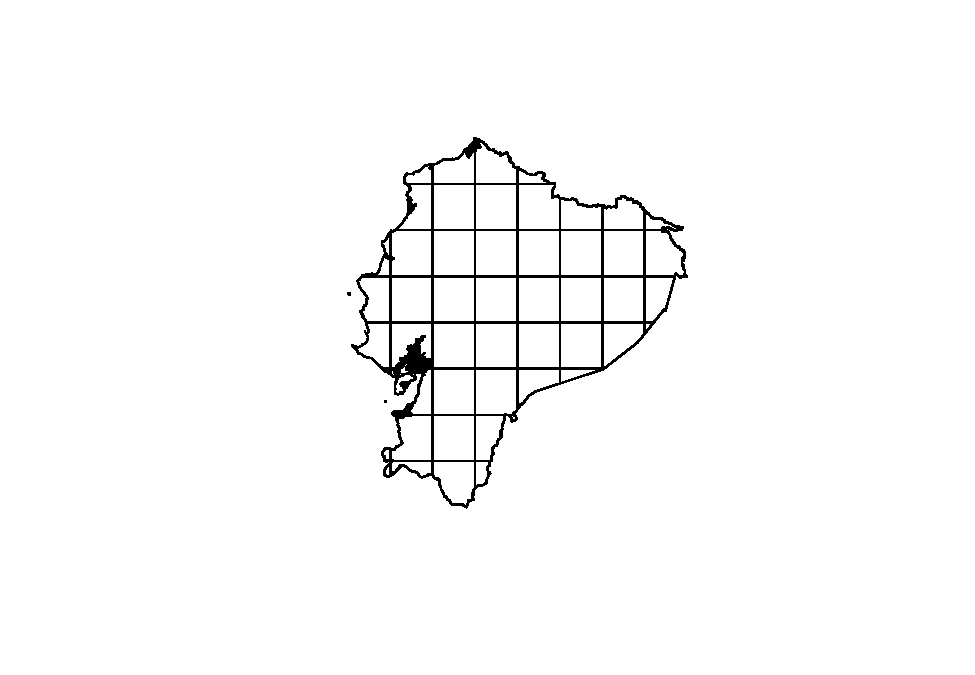
\includegraphics{_main_files/figure-latex/unnamed-chunk-21-1.pdf}
We can use \texttt{subset} to look at specific micromammals. Here's the house mouse:

\begin{Shaded}
\begin{Highlighting}[]
\CommentTok{\#Plot house mouse rainfall }
\NormalTok{houseMouse}\OtherTok{\textless{}{-}}\FunctionTok{subset}\NormalTok{(micromammals,COMMONNAME}\SpecialCharTok{==}\StringTok{"House Mouse"}\NormalTok{)}
\FunctionTok{plot}\NormalTok{(}\FunctionTok{st\_geometry}\NormalTok{(saBorders),}\AttributeTok{axes=}\NormalTok{T,}\AttributeTok{main=}\StringTok{"House Mouse"}\NormalTok{)}
\FunctionTok{plot}\NormalTok{(}\FunctionTok{st\_geometry}\NormalTok{(houseMouse),}\AttributeTok{add=}\NormalTok{T,}\AttributeTok{pch=}\DecValTok{16}\NormalTok{,}\AttributeTok{col=}\StringTok{"gray"}\NormalTok{)}
\end{Highlighting}
\end{Shaded}

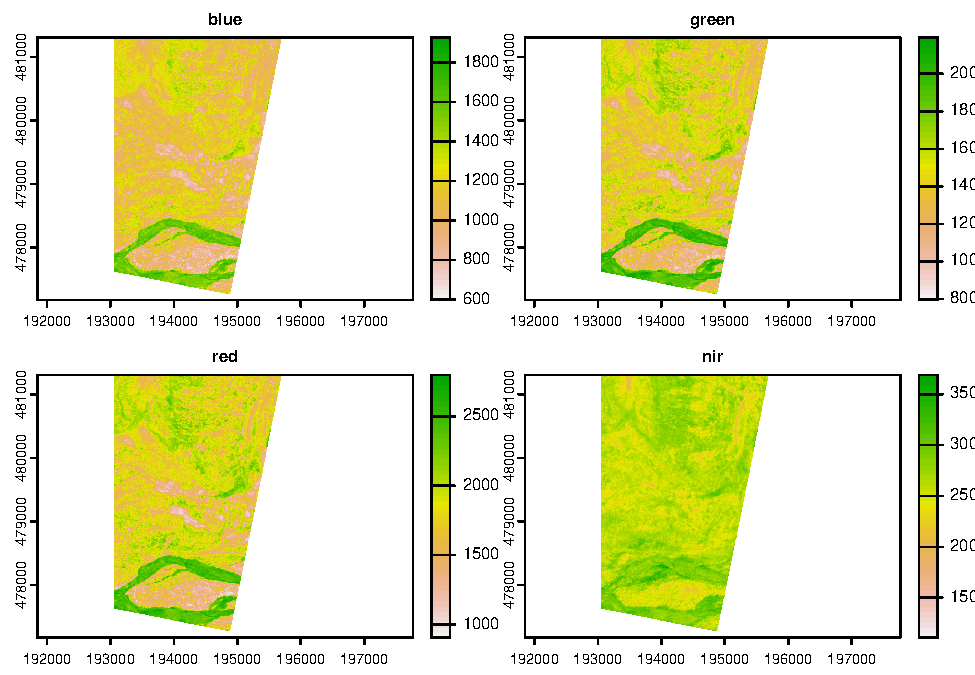
\includegraphics{_main_files/figure-latex/unnamed-chunk-22-1.pdf}
And here's the singe striped lemniscomys:

\begin{Shaded}
\begin{Highlighting}[]
\NormalTok{lemniscomys}\OtherTok{\textless{}{-}}\FunctionTok{subset}\NormalTok{(micromammals,COMMONNAME}\SpecialCharTok{==}\StringTok{"Single{-}Striped Lemniscomys"}\NormalTok{)}
\FunctionTok{plot}\NormalTok{(}\FunctionTok{st\_geometry}\NormalTok{(saBorders),}\AttributeTok{axes=}\NormalTok{T,}\AttributeTok{main=}\StringTok{"Single{-}Striped Lemniscomys"}\NormalTok{)}
\FunctionTok{plot}\NormalTok{(}\FunctionTok{st\_geometry}\NormalTok{(lemniscomys),}\AttributeTok{add=}\NormalTok{T,}\AttributeTok{pch=}\DecValTok{16}\NormalTok{,}\AttributeTok{col=}\StringTok{"brown"}\NormalTok{)}
\end{Highlighting}
\end{Shaded}

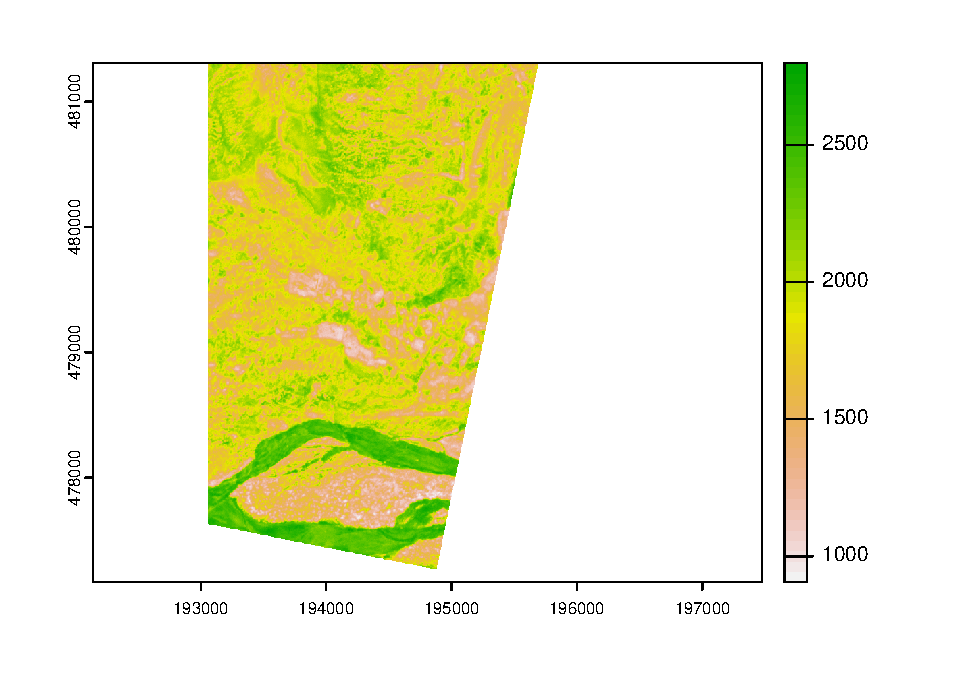
\includegraphics{_main_files/figure-latex/unnamed-chunk-23-1.pdf}

Finally, we can use this data to compare these species. Here's a \texttt{boxplot} for these two species.

\begin{Shaded}
\begin{Highlighting}[]
\FunctionTok{boxplot}\NormalTok{(houseMouse}\SpecialCharTok{$}\NormalTok{WR,lemniscomys}\SpecialCharTok{$}\NormalTok{WR,}\AttributeTok{names=}\FunctionTok{c}\NormalTok{(}\StringTok{"House Mouse"}\NormalTok{,}\StringTok{"Single{-}Striped Lemniscomys"}\NormalTok{),}\AttributeTok{ylim=}\FunctionTok{c}\NormalTok{(}\DecValTok{0}\NormalTok{,}\DecValTok{1}\NormalTok{),}\AttributeTok{ylab=}\StringTok{"\% Winter Rainfall"}\NormalTok{)}
\end{Highlighting}
\end{Shaded}

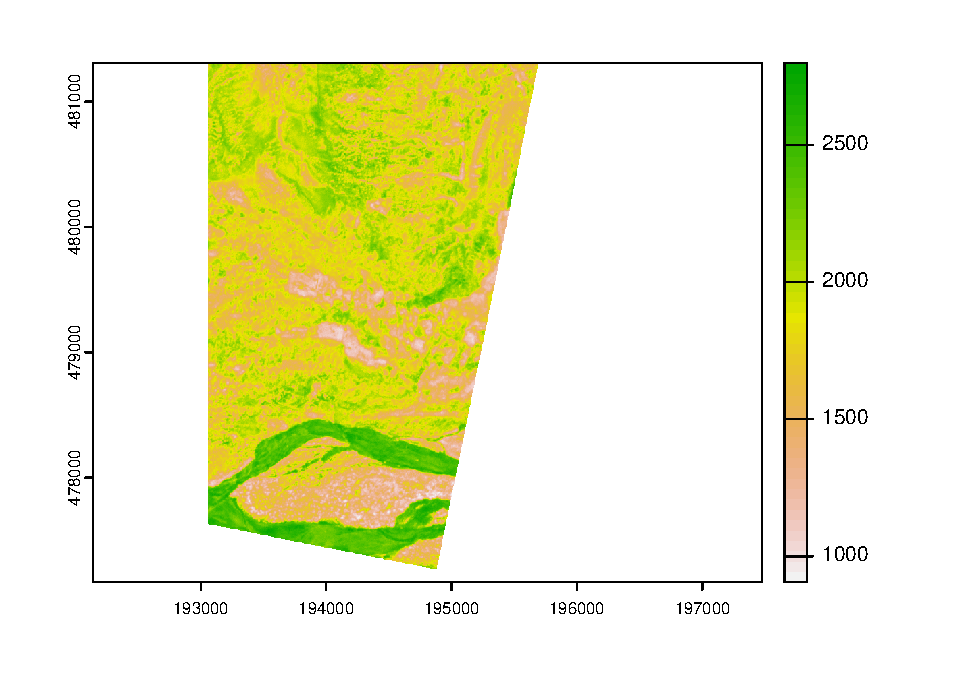
\includegraphics{_main_files/figure-latex/unnamed-chunk-24-1.pdf}

\hypertarget{bring-it-all-together}{%
\chapter{Bring it all together}\label{bring-it-all-together}}

\begin{itemize}
\tightlist
\item
  Can you subset the borders data to include only Lesotho?
\item
  Can you then spatially subset the annual and winter rainfall data? Can you get the percentage for Lesotho? The subsetting methods are up to you, but make sure you plot both with axes.
\item
  Can you get a histogram of Lesotho annual rainfall?
\end{itemize}

  \bibliography{book.bib,packages.bib}

\end{document}
